\documentclass[class=report, crop=false]{standalone}
\usepackage{../preamble}

\begin{document}
	% Specific lengths in this document
	\import{../}{default_lengths.tex}
	\tabulinesep=0.5\baselineskip
	%
	\chapter{Mã hóa dựa trên định danh}\label{chap:2}
	\section{Giới thiệu về mã hóa dựa trên định danh}
		Trong một hệ mã hóa dựa trên định danh, khi Alice muốn gửi tin cho Bob, Alice có thể dùng một chuỗi ký tự nào đó định danh Bob (ví dụ email của Bob), kết hợp với khóa công khai của một bên thứ ba được tin tưởng gọi là \textit{PKG} (private key generator) xem như khóa công khai của Bob để mã hóa thông điệp. Nhìn theo khía cạnh khác, ta có thể xem như Bob không hề có khóa công khai nào và Alice không cần khóa công khai của Bob để gửi tin, chỉ cần khóa công khai của PKG và email của Bob (tất nhiên Alice phải biết email của Bob). Kết quả là Bob không cần tự sinh khóa, Alice không cần phải lấy khóa công khai và xác thực khóa đó chính là của Bob. Nhu cầu xác thực chủ khóa không còn nữa. Hệ thống IBE giải quyết vấn đề trên một cách đơn giản và hiệu quả hơn đáng kể so với PKI.

		Cách thức vận hành của một hệ IBE được mô tả cụ thể hơn như sau, với Alice và Bob lần lượt là người gửi và người nhận:
		\vspace{-0.5cm}
		\begin{enumerate}
			\item \textit{Pha khởi tạo:} \\[0.2\baselineskip]
			Đầu tiên, PKG khởi tạo hệ thống bằng cách sinh ra một cặp khóa, tương ứng gọi là \textit{khóa công khai chủ} (master public key) và \textit{khóa bí mật chủ} (master secret key).
			\item \textit{Pha mã hóa:}
			\begin{enumerate}
				\item \textit{Xin khóa công khai chủ:} \\
				Alice gửi yêu cầu khóa công khai chủ đến PKG và nhận phản hồi. Ở đây Alice phải xác thực được khóa được nhận chính là của PKG, không phải giả mạo.
				\item \textit{Mã hóa:} \\
				Sau đó Alice sử dụng khóa công khai chủ kết hợp với định danh của Bob để mã hóa thông điệp và gửi cho Bob.
			\end{enumerate}
			\item \textit{Pha giải mã:}
			\begin{enumerate}
				\item \textit{Đăng ký:} \\
				Bob gửi yêu cầu khóa bí mật tương ứng định danh của mình đến PKG. Ở đây, khác với phía Alice, cả PKG và Bob đều phải xác thực lẫn nhau. PKG cần chắc chắn chủ thể mình đang giao tiếp là chủ sở hữu của định danh, tức là Bob. Còn Bob, giống như Alice, phải đảm bảo mình không nhận khóa từ một PKG giả mạo.
				\item \textit{Giải mã:} \\
				Sau khi nhận được khóa bí mật của mình từ PKG. Bob thực hiện giải mã gói tin từ Alice để lấy thông điệp.
			\end{enumerate}
		\end{enumerate}
		
		\begin{figure}[h]
			\captionsetup{font=normalsize}
			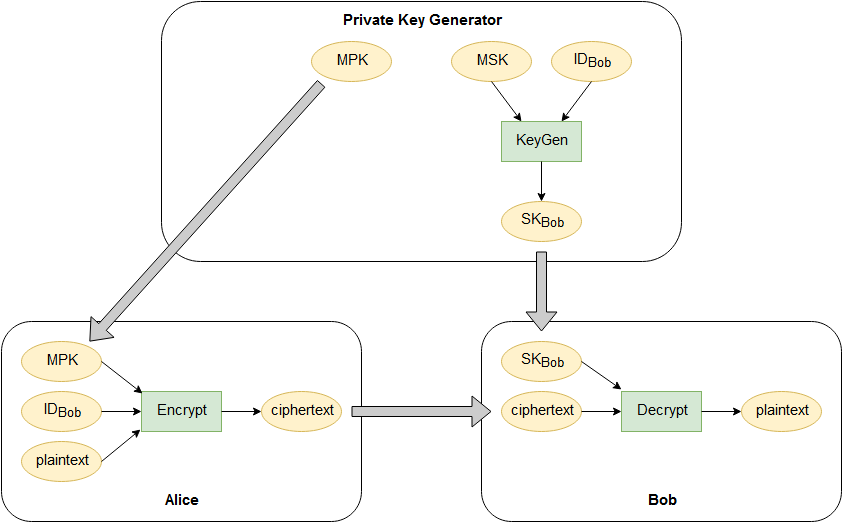
\includegraphics[width=\textwidth]{ibe_protocol.png}
			\centering
			\caption{Giao thức vận hành của một hệ IBE}
		\end{figure}
		\newpage
		Trong IBE mọi chuỗi ký tự đều có thể được dùng làm định danh, điều này mở ra rất nhiều kỹ thuật trong thiết kế hệ thống. Những kỹ thuật này sẽ được trình bày ở phần sau. Khác với hệ mã hóa khóa công khai bình thường, hệ IBE cho phép bản mã được tạo ra trước và gửi cho Bob trước cả khi Bob có khóa để giải. Quá trình giải mã có thể còn cần đến cả khóa công khai chủ, khi đó ta ngầm hiểu khóa công khai chủ được gửi kèm với khóa bí mật của Bob khi Bob đăng ký. Vì lý do này mà trong nhiều bài báo khóa công khai chủ còn được gọi là \textit{tham số công khai} (public parameters).
	%
	\section{Luận bàn về IBE và PKI}\label{fig:ibe_vs_pki}
		Phương pháp xác thực giữa các bên trong hệ IBE có thể là bất cứ phương pháp nào được dùng ở các hệ thống khác như mật khẩu, thách thức - phản hồi, v.v.. Hoặc hệ IBE có thể áp dụng đúng cách mà PKI dựa trên CA hiện giờ đang triển khai như sau: Khóa công khai chủ được phân phát đến người gửi (Alice) giống như cách chứng chỉ số của những CA gốc (root CA) được phân phát, thường là qua các kênh "chính thống" như cài sẵn trong hệ điều hành, trình duyệt web hoặc gặp trực tiếp. PKG và người đăng ký (Bob) xác thực lẫn nhau tương tự như cách giữa CA và server trong PKI khi server đăng ký chứng chỉ số. Ở cấp độ xác thực cao nhất của chứng chỉ số (như chứng chỉ Extended Validation), bắt buộc phải có sự tương tác trực tiếp (không phải từ xa) giữa hai bên. Việc vẫn còn nhu cầu xác thực trong hệ IBE cho thấy rằng IBE vẫn tương tự như PKI, ở chỗ, để đạt được sự an toàn thông tin thì tất yếu phải có những giao tiếp trực tiếp ban đầu làm cơ sở. Những giao tiếp trực tiếp này để đảm bảo thông tin có được là thực sự và chính xác.
		
		Để thấy sự khác nhau giữa IBE và PKI, vốn sử dụng mã hóa khóa công khai bình thường, ta xét ví dụ sau. Giả sử có một môi trường gồm $n$ người dùng muốn giao tiếp từ xa từng đôi một với nhau. Ở đây ta không đếm những lần giao tiếp giữa người dùng với PKG và giữa người dùng với CA, thực chất là như nhau ở cả hai loại hình. Với hệ IBE, mỗi người đều biết định danh của tất cả người khác nên \emph{không} tốn lần giao tiếp nào. Với mã hóa khóa công khai bình thường, khóa là do mỗi người tự sinh nên mỗi người phải gửi khóa công khai của mình cho từng người khác. Hạ tầng PKI chỉ đảm bảo khóa nhận được là chính chủ. Do đó cần tới $C_n^2 = n(n-1)/2$ lần giao tiếp.

		Mặt khác, trong hệ IBE, không người dùng nào có khả năng tự sinh khóa bí mật của mình mà phải nhờ đến PKG cấp cho. Điều này dẫn đến sự phụ thuộc rất lớn vào sự vận hành trung thực và tính bảo mật của PKG. Quyền hạn của PKG lớn hơn rất nhiều so với CA trong PKI. Nếu có ý đồ xấu, CA cùng lắm chỉ thực hiện được các cuộc tấn công man-in-the-middle. Tuy quyền hạn như vậy đã là không hề nhỏ nhưng không thể sánh với một PKG có thể tạo ra khóa bí mật của bất kỳ người dùng nào trong hệ thống. PKG có thể đọc bất kỳ thông điệp nào gửi cho bất kỳ ai. Tương tự với hệ \textit{chữ ký dựa trên định danh} (identity-based signature) thì PKG có thể ký bất kỳ văn bản nào nhân danh bất kỳ ai. Kể cả khi PKG vận hành trung thực thì vẫn có thể bị tấn công và mất khóa bí mật chủ dẫn đến nguy cơ mất an toàn của toàn hệ thống.

		Vì những lý do trên, hệ IBE không được dùng để thay thế PKI trên hạ tầng Internet hiện nay. IBE phù hợp hơn với những hệ thống nội bộ, đề cao sự giao tiếp tiện lợi mà trong đó sự tin tưởng tuyệt đối vào một "thực thể chính quyền" là hợp lý.
	%
	\section{Khái niệm mã hóa dựa trên định danh phân cấp}
		Trong PKI, để giảm tải cho CA gốc thì họ đưa vào thêm CA và xây dựng một kiến trúc cây giữa các CA. Trong đó CA ở nốt cha cấp chứng chỉ số cho CA ở nốt con và CA cấp dưới cùng cấp chứng chỉ số cho người dùng. Và cũng tự nhiên khi ta muốn xây dựng một kiến trúc tương tự cho hệ IBE.

		Khái niệm \textit{mã hóa dựa trên định danh phân cấp} (hierarchical identity-based encryption, từ đây gọi tắt là HIBE) được Horwitz và Lynn \cite{DBLP:conf/eurocrypt/HorwitzL02} đưa ra năm 2002, trong đó nêu ra định nghĩa hình thức và mô hình an toàn của HIBE. Trong hệ HIBE, trừ PKG gốc thì mỗi chủ thể bên dưới nó (gồm các PKG trung gian và người dùng) đều có một \textit{định danh nguyên thủy} (primitive identity). Định danh nguyên thủy của các chủ thể trực thuộc cùng một PKG (gốc hoặc trung gian) phải đôi một phân biệt. Xem PKG gốc là cấp $0$ trong cây, định danh của một chủ thể ở cấp $k \ (k > 0)$ là một bộ gồm $k$ định danh nguyên thủy của $k - 1$ chủ thể tổ tiên và chính chủ thể đó, theo thứ tự từ trên xuống. Chú ý là PKG gốc không cần có định danh hay định danh nguyên thủy, và một định danh xác định duy nhất một chủ thể trong hệ thống. Ta thấy rằng khái niệm định danh trong IBE tương ứng với định danh nguyên thủy trong HIBE. Thông thường khi khởi tạo một hệ HIBE ta phải chỉ định \textit{số cấp tối đa} cho phép trong hệ (chiều dài tối đa của định danh). Một số hệ HIBE cho phép PKG gốc có thể tăng số cấp tối đa ở thời điểm sau khởi tạo.
		
		Ví dụ, xem Nhà nước Việt Nam là PKG gốc, ở mỗi địa phương thuộc mỗi cấp hành chính có một PKG trung gian. Trường Đại học Khoa học Tự nhiên TPHCM có địa chỉ cơ sở chính là "227 Đường Nguyễn Văn Cừ, Phường 4, Quận 5, Thành phố Hồ Chí Minh". Vậy định danh nguyên thủy của trường là "227 Đường Nguyễn Văn Cừ" và định danh của trường là ("Thành phố Hồ Chí Minh", "Quận 5", "Phường 4", "227 Đường Nguyễn Văn Cừ"). Trường là nốt cấp 4 trong cây HIBE này.
		%
		\begin{figure}[h]
			\captionsetup{font=normalsize}
			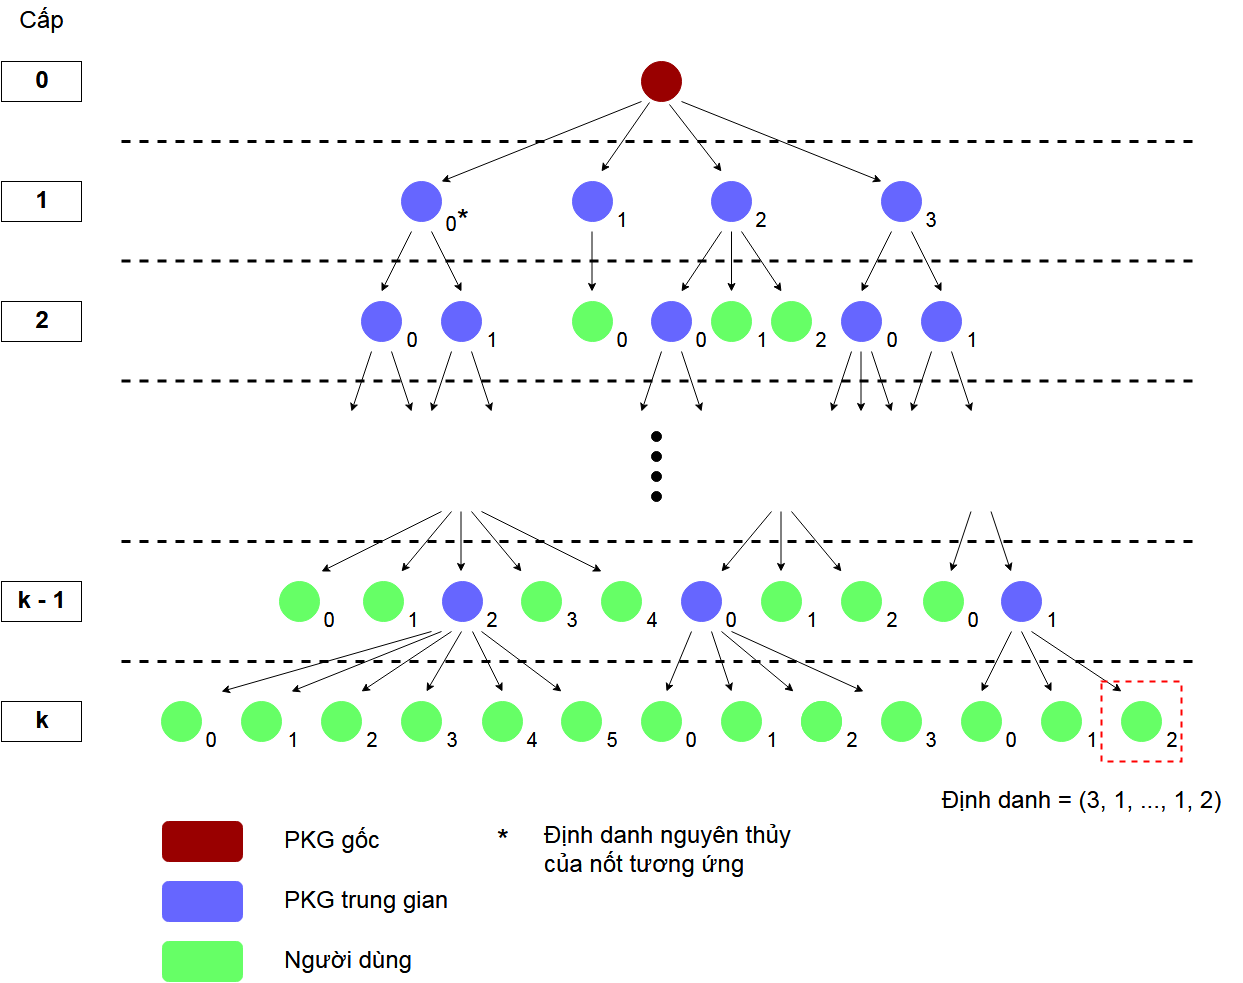
\includegraphics[width=\textwidth]{hibe_visualization.png}
			\centering
			\caption{Mã hóa dựa trên định danh phân cấp}
		\end{figure}

		Ngoài việc giảm tải công việc xác thực định danh và cấp phát khóa cho PKG gốc, kiến trúc phân cấp còn giúp giảm thiểu thiệt hại khi bị tấn công. Nếu một PKG trung gian suy yếu (bị lộ khóa) thì chỉ bộ phận bên dưới PKG đó bị mất an toàn chứ không phải toàn hệ thống. Nếu quy mô bộ phận này không lớn ta có thể tái thiết lập bộ phận này bằng cách đổi định danh.
	%
	\section{Một số tính năng cao cấp có thể có trong một hệ IBE}
		\subsection{Cơ chế sinh khóa có ngưỡng phi tương tác}
			Vì PKG nắm giữ quyền hạn rất lớn và khóa bí mật chủ nếu bị lộ sẽ gây mất an toàn cho toàn hệ thống nên Boneh và Franklin \cite{DBLP:conf/crypto/BonehF01} đã đề xuất áp dụng kỹ thuật của mật mã ngưỡng (threshold cryptography) cho IBE, cụ thể họ sử dụng biến thể của lược đồ chia sẻ thông tin mật của Shamir \cite{DBLP:journals/cacm/Shamir79} cho hệ mã của mình. Kỹ thuật ngưỡng cho phép một bí mật được ``chia'' thành $n$ phần và nếu tập hợp đủ $t$ phần (với $t \leq n$) thì bất cứ ai cũng có thể tái tạo bí mật. Sau khi chia thành các bí mật thành phần thì bí mật ban đầu phải được xóa ở tất cả mọi nơi để tránh một nơi nào đó trở thành yếu điểm của hệ thống. Trong IBE kỹ thuật ngưỡng được áp dụng cho khóa bí mật chủ. Lúc này sẽ dễ hình dung hơn nếu ta xem một PKG là một ``hội đồng'' gồm $n$ chủ thể thay vì một chủ thể đơn.
			%
			\begin{figure}[h]
				\captionsetup{font=normalsize}
				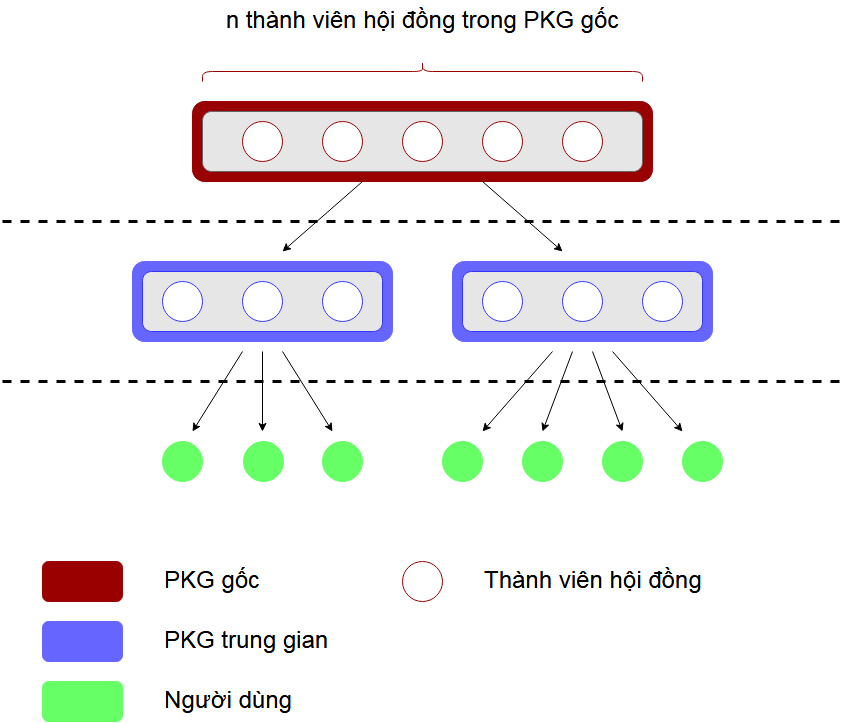
\includegraphics[width=0.9\textwidth]{threshold_ibe.png}
				\centering
				\caption{Hệ HIBE hỗ trợ sinh khóa có ngưỡng}
			\end{figure}
			
			Xét một mô hình vận hành ``ngây thơ'' như sau: Với một yêu cầu khóa bí mật từ người dùng (hoặc PKG con trong HIBE), $t$ thành viên nào đó của hội đồng sẽ hợp tác tái tạo khóa bí mật chủ, từ đó sinh ra khóa bí mật cho định danh. Tuy nhiên mô hình vận hành này có ba vấn đề:
			\vspace{-0.5cm}
			\begin{enumerate}
				\item Cần có sự giao tiếp giữa những thành viên được chọn trong hội đồng để sinh khóa, dẫn đến tốn chi phí giao tiếp (nội bộ). Giả sử nếu các thành viên là các server đặt xa nhau về mặt địa lý thì chi phí này làm chậm hệ thống rất đáng kể.
				\item Khi một thành viên được chọn không hợp tác sinh khóa một cách trung thực, khóa bí mật chủ sẽ bị tái tạo sai, dẫn đến khóa bí mật của định danh cũng bị sai theo. Nếu không có một phương thức kiểm định khóa nhận được từ PKG một cách công khai (ai cũng có thể kiểm) thì chủ thể yêu cầu khóa không có khả năng phát hiện được hành vi vi phạm này.
				\item Những thời điểm khóa bí mật chủ được tái tạo lại chính là những thời điểm trọng yếu của hệ thống, dễ trở thành mục tiêu tấn công.
			\end{enumerate}
			
			Mô hình ngưỡng được các tác giả trên đề xuất hỗ trợ xin cấp phát khóa một cách độc lập từ các thành viên PKG và kiểm định khóa công khai. Mô hình này không có sự tương tác giữa các thành viên PKG nên được gọi là cơ chế \textit{sinh khóa có ngưỡng phi tương tác} (non-interactive threshold key generation). Mô hình vận hành như sau: Mỗi người dùng khi yêu cầu khóa sẽ chọn tùy ý $t$ thành viên trong PKG rồi gửi yêu cầu đến tất cả thành viên này một cách độc lập. Sau khi nhận yêu cầu, mỗi thành viên tạo ra và phản hồi lại \textit{khóa bí mật thành phần của định danh} tương ứng với người yêu cầu, mà \emph{không} cần biết hay tương tác với các thành viên được chọn còn lại. Người dùng kiểm tra từng thành phần khóa mình nhận được có đúng hay không. Cuối cùng người dùng khi có đủ $t$ thành phần sẽ tự tạo ra khóa bí mật của chính mình.
			
			Dễ thấy rằng với mô hình vận hành này thì cả ba vấn đề trên đều được giải quyết. Việc giải quyết được vấn đề 1 ở trên có ý nghĩa rất lớn đối với khả năng mở rộng (scalability) của hệ thống. Ví dụ ta có thể đặt $t$ server ở mỗi khu vực địa lý, như vậy mọi người dùng trong một khu vực có thể được cấp phát khóa một cách ``địa phương'' mà không cần giao tiếp với bên ngoài khu vực. Tuy nhiên trong mô hình sau lại có vấn đề mới nảy sinh là gánh nặng bị tăng lên ở phía người dùng khi phải lặp lại quá trình tương tác và xác thực với nhiều server. Ở vấn đề 2 không những người dùng có thể phát hiện hành vi vi phạm mà còn biết được (những) ai là người vi phạm.

			Một điều cần nói thêm là tất cả các hệ HIBE dựa trên cặp ghép cho đến thời điểm này (ít nhất là trong phạm vi tìm hiểu của sinh viên) đều không hỗ trợ cơ chế sinh khóa có ngưỡng từ cấp 1 của cây trở xuống. Tức là trên các hệ này ta chỉ có thể ``chia'' khóa bí mật chủ (của PKG gốc), không thể ``chia'' khóa bí mật của PKG trung gian. Đây là một hạn chế bắt nguồn từ lý thuyết. Giải thích một cách đơn giản, do trong các hệ HIBE dựa trên cặp ghép, các khóa bí mật cấp dưới không tương thích về mặt đại số để áp dụng kỹ thuật của Shamir, trong khi khóa bí mật chủ thì tương thích. Sự khác nhau này sẽ được thấy rõ hơn ở chương \ref{chap:5}.
		%	
		\subsection{Giới hạn số cấp sinh khóa bí mật trong HIBE}\label{chap2:sec4:restrict_key_derivation}
			Trong một số hệ HIBE, không có sự khác nhau giữa PKG trung gian và người dùng cuối. Nghĩa là bất kỳ người dùng nào nếu muốn đều có thể bắt đầu ``kết nạp'' chủ thể bên dưới mình trong cây HIBE và ``phát hành'' khóa, miễn sao vẫn chưa vượt quá số cấp tối đa của toàn hệ HIBE. Một hệ HIBE hỗ trợ khả năng giới hạn số cấp sinh khóa cho phép PKG cấp khóa có thể hạn chế số cấp tối đa bên dưới PKG / người dùng xin khóa, mặc dù vẫn chưa chạm đến số cấp tối đa của toàn hệ HIBE. Nếu số cấp tối đa bên dưới một chủ thể bị hạn chế về $0$, chủ thể đó không thể kết nạp thêm chủ thể khác bên dưới, tức là chỉ có thể hoạt động như một người dùng cuối đúng nghĩa.
		%
		\subsection{Tính ẩn danh người dùng}
			Thông thường trong một hệ IBE, bản mã không có bất kỳ thông tin nào liên kết đến người gửi (không tính bản rõ) nên không cần phải lo ngại người gửi bị lộ. Vấn đề nằm ở tính ẩn danh của người nhận do định danh của người nhận được dùng để mã hóa. Tính ẩn danh của một hệ IBE nói rằng bất kỳ chủ thể nào ngoại trừ người gửi, người nhận và những PKG có khả năng tạo ra khóa của người nhận, cũng đều không thể phân biệt định danh nào được dùng để tạo ra bản mã, nếu không có khóa bí mật của người nhận. Cụ thể hơn, trong trò chơi an toàn giữa người tấn công và người thách thức, người tấn công tùy ý chọn ra 1 văn bản $M$ và 2 định danh $ID_0,\ ID_1$ gửi cho người thách thức. Người thách thức chọn ngẫu nhiên 1 định danh trong 2 rồi tạo bản mã $C$ của $M$ dựa trên định danh đó, sau đó gửi $C$ cho người tấn công. Nếu hệ IBE có tính ẩn danh thì người tấn công khó có thể phân biệt được $C$ được tạo ra bằng định danh nào.

			Đối với hệ HIBE thì tính ẩn danh phải được đảm bảo ở tất cả các cấp trong hệ. Tuy nhiên có những khó khăn nhất định về mặt lý thuyết để đạt được tính chất này với HIBE (xem \cite{DBLP:conf/crypto/BoyenW06}). Vẫn có hệ HIBE ẩn danh với người dùng cấp 1 nhưng không với người dùng cấp dưới đó \cite{DBLP:conf/asiacrypt/GentryS02}.
	%
	\section{Những vấn đề của IBE}
		\subsection{Phụ thuộc tuyệt đối}
			Như đã trình bày ở mục \ref{fig:ibe_vs_pki}, tất cả người dùng trong hệ IBE không thể làm gì khác ngoài tin tưởng tuyệt đối vào tính trung thực và tính kiên cố của PKG. Vấn đề này có thể được giảm thiểu một phần nhờ cơ chế sinh khóa có ngưỡng.
		%
		\subsection{Giám hộ khóa}\label{subsec:key_escrow}
			Tính \textit{giám hộ khóa} (key escrow) của một hệ mã nói chung là một khả năng cho phép khóa giải mã phải bị ``giam giữ'', và dưới một số điều kiện nhất định một chủ thể có thẩm quyền có thể suy ra hoặc yêu cầu tiết lộ khóa này. Vì PKG có khả năng sinh ra khóa bí mật của tất cả người dùng nên hệ IBE mặc nhiên sở hữu tính chất này.

			Tính giám hộ khóa là tính chất được mong muốn hay không còn tùy thuộc vào bối cảnh ứng dụng. Với mã hóa, trong một môi trường giao tiếp mà cho phép hạn chế quyền riêng tư của người dùng thì đây là tính chất mong muốn. Ví dụ một người dùng nào đó bị tình nghi phạm tội thì tòa án có thể lệnh cho PKG giải mã những tin nhắn của người dùng đó. Nhưng ngược lại với hệ chữ ký, tính giám hộ khóa lại không được mong muốn chút nào do có nhiều hơn một chủ thể (người dùng và (các) PKG) có khả năng tạo ra chữ ký hợp lệ, dẫn đến mất đi tính \textit{chống thoái thác trách nhiệm} (non-repudiation) của hệ chữ ký.

			Tương tự vấn đề phụ thuộc tuyệt đối vào PKG ở trên, cơ chế sinh khóa có ngưỡng cũng giúp hạn chế vấn đề này. Ngoài ra, đã có hệ HIBE có thiết kế cho phép với mọi chủ thể dưới PKG gốc, ngoài chủ thể đó ra thì \emph{chỉ} chủ thể cha của chủ thể đó mới có thể sinh ra khóa và giải mã bản mã gửi cho chủ thể đó \cite[mục 6.1]{DBLP:conf/asiacrypt/GentryS02}. Một cách tiếp cận khác là dùng một giao thức trao đổi khóa bình thường (chẳng hạn Diffie-Hellman) kết hợp với một hệ chữ ký dựa trên định danh, bằng cách ký lên nguyên liệu khóa gửi đi. Khóa được sử dụng để giao tiếp lúc này là \textit{khóa phiên} (session key) và khóa này \emph{không bị giám hộ}. Và trừ những chủ thể trên người nhận thì không ai khác có thể thực hiện tấn công \textit{man-in-the-middle}. Khi đó hệ thống này vận hành và có tính an toàn gần như một PKI. Chi tiết về kỹ thuật này vui lòng xem tại \cite[mục 6.2]{DBLP:conf/asiacrypt/GentryS02}. Nếu tích hợp được tất cả kỹ thuật trên vào một hệ HIBE thì tính giám hộ khóa được hạn chế rất đáng kể.
		%
		\subsection{Thu hồi khóa}\label{chap2:sec5:key_revocation}
			Với mã hóa khóa công khai bình thường, Alice trước khi gửi tin cho Bob phải kiểm tra rằng dùng khóa công khai của Bob có còn an toàn không. Trong PKI, nếu Bob phát hiện khóa riêng tư của mình bị lộ, Bob sẽ gửi yêu cầu thu hồi (revoke) chứng chỉ (tức khóa công khai) của mình lên CA. Alice chỉ cần hỏi CA (đối tượng hỏi phụ thuộc cách triển khai PKI cụ thể) khóa công khai của Bob có bị thu hồi chưa để quyết định có dùng khóa đó hay không. Điều này làm tăng thêm gánh nặng cho CA.

			Một vấn đề tương tự cũng có trong IBE. Giả sử Bob dùng email của mình là ``\texttt{bob@mail.com}'' để đăng ký với PKG. Bob phát hiện ra khóa bí mật của mình đã bị lộ. Với PKI, Bob có thể sinh ra cặp khóa mới rồi đăng ký với CA. Nhưng trong IBE khóa của Bob không do Bob tự sinh ra. Mà khóa công khai của Bob có thể xem như là khóa công khai chủ kết hợp với email của Bob. Không thể tái thiết lập toàn bộ hệ thống do chỉ mình Bob mất khóa. Vậy không lẽ Bob phải thay đổi email?

			Boneh và Franklin \cite{DBLP:conf/crypto/BonehF01} đã đề xuất giải pháp khóa ngắn hạn để giải quyết vấn đề trên: Bob được PKG cấp phát khóa theo một chu kỳ thời gian được thiết lập trước. Alice sẽ đính kèm nhãn thời gian vào email của Bob, xem toàn bộ như định danh để mã hóa. Ví dụ nếu chu kỳ là một tháng thì định danh để mã hóa là ``\texttt{bob@mail.com||05/2019}''. Đến đầu mỗi tháng Bob sẽ được PKG cấp khóa bí mật tương ứng.
			
			Cơ chế này hoạt động được là nhờ tất cả người dùng đều thống nhất chung một định dạng của định danh. Khóa bí mật của định danh chỉ hiệu lực trong một chu kỳ. Nếu khóa của Bob bị lộ thì thiệt hại sẽ nhỏ (tất cả tin gửi trong một chu kỳ) và Bob cũng không cần đổi email. Ta luôn có thể tăng giảm độ mịn thời gian tùy thuộc vào ứng dụng. Trong cơ chế này PKG không cần lưu một cơ sở dữ liệu những khóa bị thu hồi. Vì vậy Alice không cần truy vấn PKG về tình trạng khóa của Bob, đảm bảo được tính riêng tư cho hai người. Thêm nữa, cơ chế này cho phép Alice có thể gửi tin đến tương lai, tức là Alice mã hóa thông điệp bằng định danh của Bob gắn với nhãn thời gian ở tương lai. Nếu PKG vận hành đúng thì đến đúng thời điểm Bob mới có thể giải mã. Cơ chế hoạt động này đơn giản chỉ là một chiến lược đánh đổi sự hiệu quả lấy sự an toàn cho nên vẫn có những lỗ hổng. Ta vẫn chưa biết được là có giải pháp vẹn toàn nào cho vấn đề này không.
	%
	% \newpage
	\section{Định nghĩa hình thức của IBE và HIBE}
		\begin{definition}[IBE]
			Một lược đồ mã hóa dựa trên định danh là một bộ gồm bốn thuật toán \textsf{Setup, SecretKeyGen, Encrypt, Decrypt}. Trong đó:
			%
			\vspace{-0.5cm}
			\begin{itemize}
				\item[] {\sffamily\bfseries Setup($\lambda$)}
				\begin{itemize}
					\item[\textbullet] \textit{Input}: Tham số an toàn $\lambda \in \mathbb{N^*}$
					\item[\textbullet] \textit{Output}: Bộ tham số công khai $params$ và khóa bí mật chủ $msk$ \\
					Bộ tham số công khai có thể bao gồm thêm mô tả của các cấu trúc đại số được sử dụng và các không gian của bản rõ, bản mã và định danh. PKG công bố $params$ và giữ lại $msk$.
				\end{itemize}
				\item[] {\sffamily\bfseries SecretKeyGen(params, msk, ID)}
				\begin{itemize}
					\item[\textbullet] \textit{Input}: $params$, $msk$ và định danh để sinh khóa $ID$
					\item[\textbullet] \textit{Output}: Khóa bí mật $sk_{ID}$
				\end{itemize}
				\item[] {\sffamily\bfseries Encrypt(params, ID, M)}
				\begin{itemize}
					\item[\textbullet] \textit{Input}: $params$, định danh để mã hóa $ID$ và thông điệp $M$
					\item[\textbullet] \textit{Output}: Bản mã $C$
				\end{itemize}
				\item[] {\sffamily\bfseries Decrypt(params, sk\textsubscript{ID}, C)}
				\begin{itemize}
					\item[\textbullet] \textit{Input}: $params$, $sk_{ID}$ và $C$
					\item[\textbullet] \textit{Output}: $M$
				\end{itemize}
			\end{itemize}
			%
			\vspace{-\baselineskip}\indent\indent
			Thuật toán \textsf{Setup} và \textsf{SecretKeyGen} được thực thi bởi PKG, thuật toán \textsf{Encrypt} và \textsf{Decrypt} được thực thi bởi người dùng. Trừ thuật toán \textsf{Decrypt} là đơn định (deterministic), các thuật toán còn lại là ngẫu nhiên (randomized). \\ \indent
			Lược đồ phải đảm bảo tính đúng đắn, nghĩa là với mọi thông điệp $M$,
			\vspace{-\baselineskip}
			\begin{center}
				nếu \hspace{1ex} \textsf{Encrypt}$(params,\ ID,\ M) = C$ \hspace{1ex} thì \hspace{1ex} \textsf{Decrypt}$(params,\ sk_{ID},\ C) = M$.
			\end{center}
		\end{definition}
		%
		\newpage
		\begin{definition}[HIBE]
			Một lược đồ mã hóa dựa trên định danh phân cấp là một bộ gồm năm thuật toán \textsf{Setup, SecretKeyGen, Derive, Encrypt, Decrypt}. Trong đó:
			%
			\vspace{-0.5cm}
			\begin{itemize}
				\item[] {\sffamily\bfseries Setup($\lambda$, $\ell$)}
				\begin{itemize}
					\item[\textbullet] \textit{Input}: Tham số an toàn $\lambda$ và số cấp tối đa của hệ $\ell \ (\lambda, \ell \in \mathbb{N^*})$
					\item[\textbullet] \textit{Output}: Bộ tham số công khai $params$ và khóa bí mật chủ $msk$ \\
					PKG gốc công bố $params$ và giữ lại $msk$.
				\end{itemize}
				\item[] {\sffamily\bfseries SecretKeyGen(params, msk, ID)}
				\begin{itemize}
					\item[\textbullet] \textit{Input}: $params$, $msk$ và định danh để sinh khóa $ID$
					\item[\textbullet] \textit{Output}: Khóa bí mật $sk_{ID}$
				\end{itemize}
				\item[] {\sffamily\bfseries Derive(params, sk\textsubscript{ID}, ID$'$)}
				\begin{itemize}
					\item[\textbullet] \textit{Input}: $params$, khóa bí mật sk\textsubscript{ID} của định danh $ID$ và định danh để sinh khóa $ID'$ \\
					Trong đó $ID = (I_1,\ I_2, \dots,\ I_k)$ và $ID' = (I_1,\ I_2, \dots,\ I_k,\ I_{k + 1})$ với $I_j$ là các định danh nguyên thủy $(1 \leq j \leq k + 1)$. $ID$ và $ID'$ tương ứng là định danh ở cấp $k$ và $k + 1$ trong hệ (với $1 \leq k < l$).
					\item[\textbullet] \textit{Output}: Khóa bí mật $sk_{ID'}$
				\end{itemize}
				\item[] {\sffamily\bfseries Encrypt(params, ID, M)}
				\begin{itemize}
					\item[\textbullet] \textit{Input}: $params$, định danh để mã hóa $ID$ và thông điệp $M$
					\item[\textbullet] \textit{Output}: Bản mã $C$
				\end{itemize}
				\item[] {\sffamily\bfseries Decrypt(params, sk\textsubscript{ID}, C)}
				\begin{itemize}
					\item[\textbullet] \textit{Input}: $params$, $sk_{ID}$ và $C$
					\item[\textbullet] \textit{Output}: $M$
				\end{itemize}
			\end{itemize}
			%
			\vspace{-\baselineskip}\indent\indent
			Thuật toán \textsf{Setup} và \textsf{SecretKeyGen} được thực thi bởi PKG gốc, thuật toán \textsf{Derive} được thực thi bởi PKG trung gian, thuật toán \textsf{Encrypt} và \textsf{Decrypt} được thực thi bởi người dùng. Trừ thuật toán \textsf{Decrypt} là đơn định (deterministic), các thuật toán còn lại là ngẫu nhiên (randomized). \\ \indent
			Lược đồ phải đảm bảo tính đúng đắn, nghĩa là với mọi thông điệp $M$,
			\vspace{-\baselineskip}
			\begin{center}
				nếu \hspace{1ex} \textsf{Encrypt}$(params,\ ID,\ M) = C$ \hspace{1ex} thì \hspace{1ex} \textsf{Decrypt}$(params,\ sk_{ID},\ C) = M$
			\end{center}
			\vspace{-\baselineskip}
			bất kể khóa $sk_{ID}$ được sinh từ thuật toán \textsf{SecretKeyGen} hay \textsf{Derive}.
		\end{definition}
		%
		\begin{remark}
			Với một số giá trị đặc biệt của $\ell$ thì lược đồ HIBE có sự tương đồng với những lược đồ mật mã khác:
			\vspace{-0.5cm}
			\begin{itemize}
				\item[--] $\ell = 0$: Nếu ta nới lỏng định nghĩa cho phép $\ell = 0$, mã hóa với định danh rỗng và giả mã bằng khóa bí mật chủ thì lúc này lược đồ HIBE hoạt động gần như hệt lược đồ mã hóa khóa công khai. Trong đó $params$ và $msk$ tương ứng là khóa công khai và khóa riêng tư. Và không chỉ ở khía cạnh trừu tượng, nhiều lược đồ HIBE cụ thể khi cho số cấp tối đa về 0 thì ta có ngay một lược đồ mã hóa khóa công khai hoạt động tốt và an toàn.
				\item[--] $\ell = 1$: Chính là định nghĩa của IBE.
			\end{itemize}
		\end{remark}
	%
	\section{Khái niệm an toàn}
		Trong nghiên cứu mật mã tiền hiện đại, một lược đồ mật mã vẫn được xem là an toàn nếu chưa ai phát hiện ra cách tấn công nào hữu hiệu với nó. Tuy nhiên như vậy thì ta không thể biết thực sự có tồn tại cách tấn công hay không. Đến thế giới mật mã hiện đại, độ an toàn của một lược đồ phải được \emph{chứng minh} dựa trên một giả định nào đó mà được tin là đúng. Từ một tính chất được mong muốn trong một lược đồ (chẳng hạn tính bí mật), các nhà mật mã học chặt chẽ hóa tính chất này thành một trò chơi an toàn giữa người thách thức (challenger) và người tấn công (adversary). Trò chơi này liên quan mật thiết đến lược đồ. Và độ an toàn của lược đồ được định nghĩa dựa trên lợi thế (khả năng thắng trò chơi) của người tấn công. Để tiện khi gọi, cộng đồng nghiên cứu thống nhất tên gọi và ký hiệu viết tắt cho những tính chất/trò chơi này. Ví dụ như tính \textit{an toàn ngữ nghĩa} (semantic security) của một hệ mã có tên gọi tiếng Anh đầy dủ là ``(Ciphertexts) Indistinguishability under Chosen Plaintext Attack'' và viết tắt là ``IND-CPA''. Sau đây một số trò chơi an toàn sẽ được trình bày cụ thể.
		%
		\subsection{Trong IBE}
			\begin{game}{IND-ID-CCA}{Ciphertexts Indistinguishability under Adaptive Identity Chosen Ciphertext Attack}
				Xét trò chơi sau giữa người thách thức \challenger và người tấn công \adversary:
				\vspace{-1.8\baselineskip}
				\begin{itemize}[leftmargin=1.5cm, itemindent=-0.5cm]
					\item[] \textbf{Thiết lập:} \challenger chọn tham số an toàn $\lambda$ rồi chạy thuật toán \textsf{Setup}, sau đó đưa cho \adversary tham số công khai $params$.
					% 
					\item[] \textbf{Pha 1:} \adversary được thực hiện các truy vấn $q_1, q_2, ..., q_m$, trong đó $q_i$ là một trong hai loại truy vấn sau:
					\begin{itemize}
						\item[--] Truy vấn khóa bí mật của định danh $\langle ID_i \rangle$: \challenger chạy thuật toán \textsf{SecretKeyGen} để sinh khóa bí mật $sk_{ID_i}$ tương ứng với $ID_i$. \challenger phản hồi $sk_{ID_i}$ cho \adversary .
						\item[--] Truy vấn giải mã $\langle ID_i, C_i \rangle$: \challenger kiểm tra $C_i$ có phải là bản mã hợp lệ tương ứng với $ID_i$ không (nếu có thể). Nếu $C_i$ không hợp lệ thì \challenger không phản hồi. Trong trường hợp $C_i$ hợp lệ, \challenger chạy thuật toán \textsf{SecretKeyGen} để sinh khóa bí mật $sk_{ID_i}$ tương ứng với $ID_i$, sau đó chạy thuật toán \textsf{Decrypt} trên $C_i$ với khóa $sk_{ID_i}$ để lấy bản rõ. \challenger phản hồi bản rõ kết quả cho \adversary .
					\end{itemize}
					Những truy vấn này có thể được thực hiện một cách thích nghi (adaptive), tức là \adversary có thể dựa vào những kết quả truy vấn của $q_1, ..., q_{i - 1}$ để thực hiện $q_i$.
					%
					\item[] \textbf{Thử thách:} Khi mà \adversary quyết định kết thúc pha 1 thì \adversary gửi cho \challenger hai bản rõ $M_0, M_1$ có kích thước bằng nhau và một định danh $ID^*$ mà \adversary muốn được thử thách. Ràng buộc duy nhất là $ID^*$ phải không thuộc bất kỳ truy vấn khóa bí mật nào ở pha 1. Sau đó \challenger chọn ngẫu nhiên $b \in \{0, 1\}$ rồi mã hóa $M_b$ bằng thuật toán \textsf{Encrypt} trên định danh $ID^*$. \challenger gửi bản mã kết quả $C$ cho \adversary.
					%
					\item[] \textbf{Pha 2:} \adversary được tiếp tục thực hiện các truy vấn $q_{m + 1}, ..., q_{n}$ với $q_i$ là một trong hai loại:
					\begin{itemize}
						\item[--] Truy vấn khóa bí mật của định danh $\langle ID_i \rangle$ với ràng buộc $ID_i \neq ID^*$.
						\item[--] Truy vấn giải mã $\langle ID_i, C_i \rangle$ với ràng buộc $ID_i \neq ID^*$ hoặc $C_i \neq C$.
					\end{itemize}
					Tương tự pha 1, \adversary có thể thực hiện truy vấn một cách thích nghi.
					%
					\item[] \textbf{Đoán:} Cuối cùng \adversary đưa ra phán đoán $b' \in \{0, 1\}$. \adversary thắng trò chơi này nếu $b' = b$.
				\end{itemize}
				%
				\vspace{-\baselineskip}
				Ta gọi những người tấn công có quyền hạn như \adversary trong trò chơi trên là \textit{người tấn công IND-ID-CCA}. Định nghĩa \textit{lợi thế} của \adversary để tấn công hệ IBE $\mathcal{E}$ = (\textsf{Setup, SecretKeyGen, Encrypt, Decrypt}) như sau:
				\[
					\text{Adv}_{\mathcal{E, A}} = \abs{\text{Pr}(b' = b) - \frac{1}{2}}.
				\]
			\end{game}
			%
			\begin{definition}\label{def:cca}
				Cho lược đồ mã hóa dựa trên định danh \scheme và người tấn công IND-ID-CCA \adversary với thời gian tấn công bị chặn bởi $t$ và thực hiện nhiều nhất $q_{id}$ truy vấn khóa, $q_c$ truy vấn giải mã. \scheme được gọi là có mức an toàn $(t, q_{id}, q_c, \varepsilon)$-IND-ID-CCA nếu $\text{Adv}_{\mathcal{E, A}} \leq \varepsilon$. Nói cách khác, mọi người tấn công có khả năng như \adversary có lợi thế nhiều nhất là $\varepsilon$ để tấn công \scheme.
			\end{definition}
			%
			\begin{game}{IND-ID-CPA}{Ciphertexts Indistinguishability under Adaptive Identity Chosen Plaintext Attack}
				Hầu hết tương tự trò chơi IND-ID-CCA, chỉ khác ở chỗ người tấn công không được phép thực hiện truy vấn giải mã ở pha 1 và 2.
			\end{game}
			%
			\begin{definition}\label{def:cpa}
				Ta nói lược đồ \scheme có mức an toàn $(t, q_{id}, \varepsilon)$-IND-ID-CPA nếu \scheme có mức an toàn $(t, q_{id}, 0, \varepsilon)$-IND-ID-CCA.
			\end{definition}
			%
			\begin{game}{IND-sID-CPA/CCA}{Ciphertexts Indistinguishability under Selective Identity Chosen Plaintext/Ciphertext Attack}
				Ta thay đổi trò chơi IND-ID-CCA như sau: \\[0.2\baselineskip] \indent
				Người tấn công \adversary phải công bố định danh mục tiêu $ID^*$ từ đầu trò chơi (trước pha thiết lập) thay vì ở pha thử thách. Người thách thức \challenger thực hiện pha thiết lập một cách độc lập với lựa chọn của \adversary (\challenger xem như mình không hề biết $ID^*$). Ở pha 1 \adversary bị ràng buộc không được truy vấn khóa bí mật của $ID^*$, \challenger vẫn được phép truy vấn giải mã trên $ID^*$. Các pha còn lại không đổi. Trò chơi sau thay đổi được gọi là IND-sID-CCA. \\[0.2\baselineskip] \indent
				Thay đổi tương tự với trò chơi IND-ID-CPA ta được trò chơi IND-sID-CPA. \\ \indent
				Định nghĩa an toàn IND-sID-CPA/CCA tương tự như định nghĩa \ref{def:cca} và \ref{def:cpa}. Ta cũng gọi một hệ IBE an toàn trong trò chơi \adversary được quyền chọn định danh mục tiêu ở pha thử thách là \textit{an toàn định danh thích nghi} (adaptive identity secure) hay \textit{an toàn hoàn toàn} (fully secure), và gọi hệ an toàn trong trò chơi \adversary phải công bố trước từ đầu là \textit{an toàn định danh chọn lọc} (selective identity secure).
			\end{game}
			%
			\vspace{\baselineskip}
			\begin{remark}
				Định nghĩa IND-ID-CCA rất gần với định nghĩa IND-CCA - mức an toàn được xem là chuẩn mực đối với mã hóa không công khai. Chỉ có hai điểm khác là có thêm truy vấn khóa bí mật và người tấn công được chọn khóa công khai (định danh) mục tiêu, thay vì khóa công khai được chọn ngẫu nhiên. Bối cảnh đa người dùng của IBE dẫn đến có nhiều khóa công khai cho người tấn công lựa chọn. Định nghĩa an toàn trong IBE cũng phải mạnh hơn, để trong trường hợp người tấn công có trong tay khóa bí mật của một bộ phận người dùng thì phần người dùng còn lại của hệ thống vẫn được đảm bảo an toàn.
			\end{remark}
		%
		\subsection{Trong HIBE}
			\begin{definition}
				Cho hai định danh $ID$ và $ID'$, trong đó $ID = (I_1, I_2, ..., I_n)$. $ID'$ được gọi là một \textit{tiền tố} của $ID$ nếu tồn tại số nguyên dương $m \leq n$ sao cho $ID' = (I_1, ..., I_m)$.
			\end{definition}
			\begin{game}{IND-sID-CCA}{Ciphertexts Indistinguishability under Selective Identity Chosen Ciphertext Attack}
				Xét trò chơi sau giữa người thách thức \challenger và người tấn công \adversary:
				\vspace{-1.8\baselineskip}
				\begin{itemize}[leftmargin=1.5cm, itemindent=-0.5cm]
					\item[] \textbf{Khởi đầu:} \adversary công bố định danh muốn tấn công $ID^*$.
					\item[] \textbf{Thiết lập:} \challenger chọn tham số an toàn $\lambda$, số cấp tối đa $\ell$ rồi chạy thuật toán \textsf{Setup}, sau đó đưa cho \adversary tham số công khai $params$.
					% 
					\item[] \textbf{Pha 1:} \adversary được thực hiện các truy vấn $q_1, q_2, ..., q_m$, trong đó $q_i$ là một trong hai loại truy vấn sau:
					\begin{itemize}
						\item[--] Truy vấn khóa bí mật của định danh $\langle ID_i \rangle$ với ràng buộc $ID_i$ không là tiền tố của $ID^*$: \challenger chạy thuật toán \textsf{SecretKeyGen} để sinh khóa bí mật $sk_{ID_i}$ tương ứng với $ID_i$. \challenger phản hồi $sk_{ID_i}$ cho \adversary .
						\item[--] Truy vấn giải mã $\langle ID_i, C_i \rangle$ ($ID_i$ được phép là tiền tố của $ID^*$): \challenger kiểm tra $C_i$ có phải là bản mã hợp lệ tương ứng với $ID_i$ không (nếu có thể). Nếu $C_i$ không hợp lệ thì \challenger không phản hồi. Trong trường hợp $C_i$ hợp lệ, \challenger chạy thuật toán \textsf{SecretKeyGen} để sinh khóa bí mật $sk_{ID_i}$ tương ứng với $ID_i$, sau đó chạy thuật toán \textsf{Decrypt} trên $C_i$ với khóa $sk_{ID_i}$ để lấy bản rõ. \challenger phản hồi bản rõ kết quả cho \adversary .
					\end{itemize}
					Những truy vấn này có thể được thực hiện một cách thích nghi (adaptive), tức là \adversary có thể dựa vào những kết quả truy vấn của $q_1, ..., q_{i - 1}$ để thực hiện $q_i$.
					%
					\item[] \textbf{Thử thách:} Khi mà \adversary quyết định kết thúc pha 1 thì \adversary gửi cho \challenger hai bản rõ $M_0, M_1$ có kích thước bằng nhau mà \adversary muốn được thử thách. Sau đó \challenger chọn ngẫu nhiên $b \in \{0, 1\}$ rồi mã hóa $M_b$ bằng thuật toán \textsf{Encrypt} trên định danh $ID^*$. \challenger gửi bản mã kết quả $C$ cho \adversary.
					%
					\item[] \textbf{Pha 2:} \adversary được tiếp tục thực hiện các truy vấn $q_{m + 1}, ..., q_{n}$ với $q_i$ là một trong hai loại:
					\begin{itemize}
						\item[--] Truy vấn khóa bí mật của định danh $\langle ID_i \rangle$ với ràng buộc $ID_i$ không là tiền tố của $ID^*$.
						\item[--] Truy vấn giải mã $\langle ID_i, C_i \rangle$ với ràng buộc $ID_i$ không là tiền tố của $ID^*$ hoặc $C_i \neq C$.
					\end{itemize}
					Tương tự pha 1, \adversary có thể thực hiện truy vấn một cách thích nghi.
					%
					\item[] \textbf{Đoán:} Cuối cùng \adversary đưa ra phán đoán $b' \in \{0, 1\}$. \adversary thắng trò chơi này nếu $b' = b$.
				\end{itemize}
				%
				\vspace{-\baselineskip}
				Định nghĩa lợi thế của \adversary để tấn công hệ HIBE $\mathcal{E}$ = (\textsf{Setup, SecretKeyGen, Derive, Encrypt, Decrypt}) như sau:
				\[
					\text{Adv}_{\mathcal{E, A}} = \abs{\text{Pr}(b' = b) - \frac{1}{2}}.
				\]
			\end{game}
			%
			\begin{definition}
				Cho lược đồ mã hóa dựa trên định danh phân cấp \scheme có số cấp tối đa $\ell$ và người tấn công IND-sID-CCA \adversary với thời gian tấn công bị chặn bởi $t$ và thực hiện nhiều nhất $q_{id}$ truy vấn khóa, $q_c$ truy vấn giải mã. \scheme được gọi là có mức an toàn $(t, q_{id}, q_c, \ell, \varepsilon)$-IND-sID-CCA nếu $\text{Adv}_{\mathcal{E, A}} \leq \varepsilon$. Nói cách khác, mọi người tấn công có khả năng như \adversary có lợi thế nhiều nhất là $\varepsilon$ để tấn công \scheme.
			\end{definition}
			%
			Ta có thể xây dựng trò chơi và định nghĩa an toàn phiên bản CPA và phiên bản chọn định danh mục tiêu sau (adaptive identity) hoàn toàn tương tự như với IBE.

			Thông thường để dễ cho việc chứng minh an toàn, những nhà mật mã học mong muốn xây dựng hệ HIBE có tính chất \textit{độc lập với lịch sử sinh khóa} (delegation history independence). Tính chất này nói rằng khóa bí mật của một định danh không làm lộ quá trình sinh nên khóa đó (khóa được sinh bởi chủ thể tổ tiên nào, bởi thuật toán \textsf{SecretKeyGen} hay thuật toán \textsf{Derive}). Do thuật toán \textsf{SecretKeyGen} và \textsf{Derive} là thuật toán ngẫu nhiên nên có thể có nhiều khóa bí mật hợp lệ ứng với một định danh. Tính độc lập với lịch sử sinh khóa sẽ được thỏa mãn nếu khóa bí mật sinh bởi thuật toán \textsf{SecretKeyGen} và \textsf{Derive} có cùng phân phối xác suất. Vì vậy trong thuật toán \textsf{Derive} có thêm một số bước để tái tạo độ ngẫu nhiên (rerandomize).
			
			Một vấn đề nữa về tính an toàn cần được quan tâm là tính \textit{chống cấu kết} (collusion-resistance), tức là những chủ thể bên dưới dù có hợp sức lại với nhau cũng không thể suy ra khóa bí mật của PKG bên trên. Một hệ (H)IBE được gọi là \textit{chống cấu kết hoàn toàn} (fully collusion-resistant) nếu tất cả chủ thể bên dưới cấu kết lại cũng không thể suy ra khóa của PKG; và được gọi là \textit{chống cấu kết một phần} (partial collusion-resistant) nếu số lượng chủ thể cấu kết vượt qua một ngưỡng nào đó thì có thể suy ra được khóa của PKG, dưới ngưỡng đó thì không. Ở đây sinh viên không trình bày trò chơi an toàn về tính chống cấu kết. Trong những hệ HIBE dựa trên cặp ghép thì tính chất này thường dễ đạt được nhờ kỹ thuật tái tạo độ ngẫu nhiên nói trên.
	%
	\section{Những bài toán khó và giả định}
		Cho đến thời điểm này toàn bộ các hệ IBE đều dựa trên cặp ghép song tuyến tính, thặng dư bình phương hoặc dàn. Mặc dù hệ IBE xây dựng trên thặng dư bình phương \cite{DBLP:conf/ima/Cocks01} xuất hiện cùng lúc với hệ của Boneh và Franklin \cite{DBLP:conf/crypto/BonehF01} nhưng do độ hiệu quả không cao nên đến giờ vẫn không được chú trọng nghiên cứu. Trong khi đó nghiên cứu IBE trên cặp ghép gần như đã đến mức bão hòa. Vài năm gần đây xuất hiện các hệ dựa trên dàn. Dàn cho thấy được rất nhiều tiềm năng và nhiều nhà mật mã học đang xây dựng lại những kết quả đã đạt được với cặp ghép cho dàn. Dù vậy sinh viên nhìn nhận rằng IBE dựa trên dàn vẫn còn chưa đủ độ chín để tới được ứng dụng và quyết định chọn tìm hiểu IBE dựa trên cặp ghép. \\ \indent
		Sau đây là định nghĩa cặp ghép được dùng trong mật mã.
		%
		\begin{definition}
			Cho các nhóm nhân $\mathbb{G}_1$, $\mathbb{G}_2$, $\mathbb{G}_T$ thỏa $|\mathbb{G}_1| = |\mathbb{G}_2| = |\mathbb{G}_T| = p$ với $p$ là số nguyên tố. Ánh xạ $e: \mathbb{G}_1 \times \mathbb{G}_2 \rightarrow \mathbb{G}_T$ được gọi là \textit{cặp ghép (song tuyến tính)} nếu thỏa tất cả tính chất sau:
			\vspace{-0.5cm}
			\begin{enumerate}[leftmargin=1.5cm, itemindent=-0.5cm]
				\item \textit{Song tuyến tính} (bilinear):
				\[
					\text{Với mọi}\quad a \in \mathbb{G}_1,\ b \in \mathbb{G}_2,\ x, y \in \mathbb{Z}_p \quad \text{ta có} \quad e(a^x, b^y) = e(a, b)^{xy}.
				\]
				\item \textit{Không suy biến} (non-degenerate):
				\[
					\text{Tồn tại}\quad a \in \mathbb{G}_1,\ b \in \mathbb{G}_2 \quad \text{sao cho} \quad e(a, b) \neq 1.
				\]
				\item \textit{Khả tính} (computable): \\
				Tồn tại một thuật toán hiệu quả (thời gian đa thức) để tính $e(a, b)$ với mọi $a \in \mathbb{G}_1,\ b \in \mathbb{G}_2$.
			\end{enumerate} \par
			Ta gọi $e$ là \textit{cặp ghép đối xứng} khi $\mathbb{G}_1 = \mathbb{G}_2$ và là \textit{cặp ghép bất đối xứng} trong trường hợp ngược lại.
		\end{definition}
		%
		\begin{remark}
			\leavevmode \vspace{-\baselineskip}
			\begin{enumerate}[label=(\roman*), leftmargin=1cm]
				\item Do $\mathbb{G}_1$ (tương ứng $\mathbb{G}_2$, $\mathbb{G}_T$) có cấp là số nguyên tố nên mọi phần tử khác $1$ trong $\mathbb{G}_1$ (tương ứng $\mathbb{G}_2$, $\mathbb{G}_T$) đều là phần tử sinh của nhóm.
				\item Nếu $a$ và $b$ lần lượt là phần tử sinh của $\mathbb{G}_1$ và $\mathbb{G}_2$ thì ta có $e(a, b)$ là phần tử sinh của $\mathbb{G}_T$. \label{remark:pairing.2}
			\end{enumerate}
		\end{remark}
		%
		Để chứng minh một lược đồ mật mã thỏa tính chất an toàn chỉ định, thông thường ta phải dựa trên giả định độ khó của một bài toán nào đó. Định lý về độ an toàn của lược đồ thường có dạng như sau: ``Nếu bài toán $\mathcal{P}$ là khó thì lược đồ thỏa tính chất an~toàn''. Quá trình chứng minh thường theo chiều ngược lại (phản đảo). Nghĩa là nếu tồn tại một người tấn công (thuật toán) phá được lược đồ thì bằng quy dẫn (reduction) ta xây dựng được một thuật toán hiệu quả để giải bài toán $\mathcal{P}$. Bài toán càng khó thì lược đồ mật mã xây dựng dựa trên độ khó của nó càng an toàn. Vì thế các nhà mật mã học luôn muốn xây dựng lược đồ trên bài toán càng khó càng tốt để lược đồ của mình khó bị phá.
		
		Giả sử ta có thuật toán giải bài toán $\mathcal{P}_1$, xem như một hộp đen. Trên đó ta xây dựng được một thuật toán giải bài toán $\mathcal{P}_2$ bằng một số lần gọi hộp đen này đủ ít (chặn trên bởi một hàm đa thức nào đó). Sau đó nếu ta hiện thực hóa được hộp đen này bằng một thuật toán thời gian đa thức giải $\mathcal{P}_1$ thì đồng thời ta cũng nhận được một thuật toán thời gian đa thức giải $\mathcal{P}_2$. Thuật toán giải $\mathcal{P}_2$ từ hộp đen giải $\mathcal{P}_1$ ở trên, nói một cách phi hình thức, chính là một \textit{phép quy dẫn thời gian đa thức} (polynomial-time reduction) từ $\mathcal{P}_2$ về $\mathcal{P}_1$. Song song việc đi tìm thuật toán hiệu quả giải một bài toán nào đó, các nhà khoa học máy tính luôn cố gắng xây dựng phép quy dẫn giữa các bài toán, với mục đích vẽ lên bức tranh toàn cảnh liên hệ độ khó của các bài toán. Nếu giải được $\mathcal{P}_1$ thì xem như ta làm được một công đôi việc -- giải được cả hai. Vì thế cũng có thể xem như rằng việc giải được $\mathcal{P}_1$ ít nhất khó bằng việc giải được $\mathcal{P}_2$. Nói cách khác, $\mathcal{P}_1$ khó giải hơn $\mathcal{P}_2$.

		Tiếp theo sinh viên xin giới thiệu một vài bài toán phổ biến được dùng làm nền tảng độ an toàn cho các lược đồ mật mã.
		%
		\subsection{Những bài toán trên một nhóm}
			\begin{supposition}{cho bài toán DL, C-DH, D-DH}
				Cho $\mathbb{G}$ là nhóm cyclic hữu hạn với $|\mathbb{G}| = n$.
			\end{supposition}
			%
			Ký hiệu \hspace{1ex} $r \xleftarrow{R} S$ \hspace{1ex} mang ý nghĩa $r$ được chọn ngẫu nhiên theo phân phối đều từ tập S hữu hạn.
			%
			\begin{problem}{Discrete Logarithm}{DL}
				Bài toán DL trong $\mathbb{G}$ được phát biểu như sau:
				\vspace{-\baselineskip}
				\begin{itemize}[leftmargin=1.5cm, itemindent=-0.5cm]
					\item[] \textit{Input:} $g, g^x$ \\
					Trong đó: \vspace{-\baselineskip}
					\begin{align*}
						g &\xleftarrow{R} \{ a \in \mathbb{G}\ | \ \langle a \rangle = \mathbb{G} \} \\
						x &\xleftarrow{R} \mathbb{Z}_n
					\end{align*}
					\item[] \textit{Output:} $x$
				\end{itemize}
				%
				\vspace{-\baselineskip}\par
				Lợi thế của thuật toán \algo trong việc giải bài DL trong $\mathbb{G}$ được định nghĩa là
				\[
					\text{Adv}_{\mathcal{A}}^{\text{DL}} = \text{Pr}\bigg[ \ \mathcal{A}\Big(g, g^x \Big) = x \ \bigg].
				\] \indent
				Ta nói giả định $(t, \varepsilon)$-DL là đúng trong $\mathbb{G}$ nếu mọi thuật toán chạy trong thời gian $t$ đều có lợi thế nhiều nhất là $\varepsilon$ trong việc giải bài DL trong $\mathbb{G}$.
			\end{problem}
			%
			\begin{problem}{Computational Diffie-Hellman}{C-DH}
				Bài toán C-DH trong $\mathbb{G}$ được phát biểu như sau:
				\vspace{-\baselineskip}
				\begin{itemize}[leftmargin=1.5cm, itemindent=-0.5cm]
					\item[] \textit{Input:} $g, g^x, g^y$ \\
					Trong đó: \vspace{-\baselineskip}
					\begin{align*}
						g 		&\xleftarrow{R} \{ a \in \mathbb{G}\ | \ \langle a \rangle = \mathbb{G} \} \\
						x, y 	&\xleftarrow{R} \mathbb{Z}_n
					\end{align*}
					\item[] \textit{Output:} $g^{xy}$
				\end{itemize}
				%
				\vspace{-\baselineskip}\par
				Lợi thế của thuật toán \algo trong việc giải bài C-DH trong $\mathbb{G}$ được định nghĩa là
				\[
					\text{Adv}_{\mathcal{A}}^{\text{C-DH}} = \text{Pr}\bigg[ \ \mathcal{A}\Big(g, g^x, g^y \Big) = g^{xy} \ \bigg].
				\] \indent
				Ta nói giả định $(t, \varepsilon)$-C-DH là đúng trong $\mathbb{G}$ nếu mọi thuật toán chạy trong thời gian $t$ đều có lợi thế nhiều nhất là $\varepsilon$ trong việc giải bài C-DH trong $\mathbb{G}$.
			\end{problem}
			%
			\begin{problem}{Decisional Diffie-Hellman}{D-DH}
				Bài toán D-DH trong $\mathbb{G}$ được phát biểu như sau:
				\vspace{-\baselineskip}
				\begin{itemize}[leftmargin=1.5cm, itemindent=-0.5cm]
					\item[] \textit{Input:} $g, g^x, g^y, u$ \\
					Trong đó: \vspace{-\baselineskip}
					\begin{align*}
						g 		&\xleftarrow{R} \{ a \in \mathbb{G}\ | \ \langle a \rangle = \mathbb{G} \} 	\\
						x, y 	&\xleftarrow{R} \mathbb{Z}_n 												\\
						\sigma 	&\xleftarrow{R} \mathbb{G}													\\
						b 		&\xleftarrow{R} \{ 0, 1 \}
					\end{align*}
					\[
						u = \begin{cases}
							\sigma 	&\text{nếu}\quad b = 0 \\
							g^{xy} 	&\text{nếu}\quad b = 1
						\end{cases}
					\]
					\item[] \textit{Output:}
					\[
						\begin{cases}
							0 &\text{nếu}\quad u \neq g^{xy} \\
							1 &\text{nếu}\quad u = g^{xy}
						\end{cases}
					\]
				\end{itemize}
				%
				\vspace{-\baselineskip}\par
				Lợi thế của thuật toán \algo trong việc giải bài D-DH trong $\mathbb{G}$ được định nghĩa là
				\[
					\text{Adv}_{\mathcal{A}}^{\text{D-DH}} = \Bigg|\ \text{Pr}\bigg[ \ \mathcal{A}\Big(g, g^x, g^y, g^{xy} \Big) = 1 \ \bigg] - \text{Pr}\bigg[ \ \mathcal{A}\Big(g, g^x, g^y, \sigma \Big) = 1 \ \bigg]\ \Bigg|.
				\] \indent
				Ta nói giả định $(t, \varepsilon)$-D-DH là đúng trong $\mathbb{G}$ nếu mọi thuật toán chạy trong thời gian $t$ đều có lợi thế nhiều nhất là $\varepsilon$ trong việc giải bài D-DH trong $\mathbb{G}$.
			\end{problem}
		%
		\subsection{Những bài toán trên cặp ghép đối xứng}
			\begin{supposition}{cho bài toán BDH, BDHE, BDHI phiên bản đối xứng}
				Cho $\mathbb{G}$ và $\mathbb{G}_T$ là hai nhóm cyclic hữu hạn thỏa $|\mathbb{G}| = |\mathbb{G}_T| = p$ với $p$ là số nguyên tố, cặp ghép $e: \mathbb{G} \times \mathbb{G} \rightarrow \mathbb{G}_T$.
			\end{supposition}
			%
			\begin{problem}{Computational Bilinear Diffie-Hellman}{C-BDH}
				Bài toán C-BDH (phiên bản đối xứng) trong $(\mathbb{G}, \mathbb{G}_T, e)$ được phát biểu như sau:
				\vspace{-\baselineskip}
				\begin{itemize}[leftmargin=1.5cm, itemindent=-0.5cm]
					\item[] \textit{Input:} $g, g^x, g^y, g^z$ \\
					Trong đó: \vspace{-\baselineskip}
					\begin{align*}
						g 			&\xleftarrow{R} \mathbb{G}^* \quad (\mathbb{G} \setminus \{1\}) \\
						x, y, z 	&\xleftarrow{R} \mathbb{Z}_p
					\end{align*}
					\item[] \textit{Output:} $e(g, g)^{xyz}$
				\end{itemize}
				%
				\vspace{-\baselineskip}\par
				Lợi thế của thuật toán \algo trong việc giải bài C-BDH trong $(\mathbb{G}, \mathbb{G}_T, e)$ được định nghĩa là
				\[
					\text{Adv}_{\mathcal{A}}^{\text{C-BDH}} = \text{Pr}\bigg[ \ \mathcal{A}\Big(g, g^x, g^y, g^z \Big) = e(g, g)^{xyz} \ \bigg].
				\] \indent
				Ta nói giả định $(t, \varepsilon)$-C-BDH là đúng trong $(\mathbb{G}, \mathbb{G}_T, e)$ nếu mọi thuật toán chạy trong thời gian $t$ đều có lợi thế nhiều nhất là $\varepsilon$ trong việc giải bài C-BDH trong $(\mathbb{G}, \mathbb{G}_T, e)$.
			\end{problem}
			%
			\begin{problem}{Computational Bilinear Diffie-Hellman Exponent}{C-BDHE}
				Bài toán $\ell$-C-BDHE (phiên bản đối xứng) $(\ell \geq 1)$ trong $(\mathbb{G}, \mathbb{G}_T, e)$ được phát biểu như sau:
				\vspace{-\baselineskip}
				\begin{itemize}[leftmargin=1.5cm, itemindent=-0.5cm]
					\item[] \textit{Input:} $g, g^\alpha, g^{(\alpha^2)}, ..., g^{(\alpha^\ell)}, h$ \\
					Trong đó: \vspace{-\baselineskip}
					\begin{align*}
						g, h 	&\xleftarrow{R} \mathbb{G}^* \\
						\alpha 	&\xleftarrow{R} \mathbb{Z}_p^*
					\end{align*}
					\item[] \textit{Output:} $e(g, h)^{(\alpha^{\ell + 1})}$
				\end{itemize}
				%
				\vspace{-\baselineskip}\par
				Lợi thế của thuật toán \algo trong việc giải bài $\ell$-C-BDHE trong $(\mathbb{G}, \mathbb{G}_T, e)$ được định nghĩa là
				\[
					\text{Adv}_{\mathcal{A}}^{\text{C-BDHE}} = \text{Pr}\bigg[ \ \mathcal{A}\Big(g, g^\alpha, g^{(\alpha^2)}, ..., g^{(\alpha^\ell)}, h \Big) = e(g, h)^{(\alpha^{\ell + 1})} \ \bigg].
				\] \indent
				Ta nói giả định $(t, \varepsilon, \ell)$-C-BDHE là đúng trong $(\mathbb{G}, \mathbb{G}_T, e)$ nếu mọi thuật toán chạy trong thời gian $t$ đều có lợi thế nhiều nhất là $\varepsilon$ trong việc giải bài $\ell$-C-BDHE trong $(\mathbb{G}, \mathbb{G}_T, e)$.
			\end{problem}
			%
			\begin{problem}{Computational Bilinear Diffie-Hellman Inversion}{C-BDHI}
				Bài toán $\ell$-C-BDHI (phiên bản đối xứng) $(\ell \geq 1)$ trong $(\mathbb{G}, \mathbb{G}_T, e)$ được phát biểu như sau:
				\vspace{-\baselineskip}
				\begin{itemize}[leftmargin=1.5cm, itemindent=-0.5cm]
					\item[] \textit{Input:} $g, g^\alpha, g^{(\alpha^2)}, ..., g^{(\alpha^\ell)}, h$ \\
					Trong đó: \vspace{-\baselineskip}
					\begin{align*}
						g, h 	&\xleftarrow{R} \mathbb{G}^* \\
						\alpha 	&\xleftarrow{R} \mathbb{Z}_p^*
					\end{align*}
					\item[] \textit{Output:} $e(g, h)^{1/\alpha}$
				\end{itemize}
				%
				\vspace{-\baselineskip}\par
				Lợi thế của thuật toán \algo trong việc giải bài $\ell$-C-BDHI trong $(\mathbb{G}, \mathbb{G}_T, e)$ được định nghĩa là
				\[
					\text{Adv}_{\mathcal{A}}^{\text{C-BDHI}} = \text{Pr}\bigg[ \ \mathcal{A}\Big(g, g^\alpha, g^{(\alpha^2)}, ..., g^{(\alpha^\ell)}, h \Big) = e(g, h)^{1/\alpha} \ \bigg].
				\] \indent
				Ta nói giả định $(t, \varepsilon, \ell)$-C-BDHI là đúng trong $(\mathbb{G}, \mathbb{G}_T, e)$ nếu mọi thuật toán chạy trong thời gian $t$ đều có lợi thế nhiều nhất là $\varepsilon$ trong việc giải bài $\ell$-C-BDHI trong $(\mathbb{G}, \mathbb{G}_T, e)$.
			\end{problem}
		%
		\subsection{Những bài toán trên cặp ghép bất đối xứng}
			\begin{supposition}{cho bài toán BDH, coBDH, BDHE, BDHI phiên bản bất đối xứng}
				Cho $\mathbb{G}_1$, $\mathbb{G}_2$, $\mathbb{G}_T$ là các nhóm cyclic hữu hạn thỏa $|\mathbb{G}_1| = |\mathbb{G}_2| = |\mathbb{G}_T| = p$ với $p$ là số nguyên tố, cặp ghép $e: \mathbb{G}_1 \times \mathbb{G}_2 \rightarrow \mathbb{G}_T$.
			\end{supposition}
			%
			\begin{problem}{Computational Bilinear Diffie-Hellman}{C-BDH}
				Bài toán C-BDH (phiên bản bất đối xứng) trong $(\mathbb{G}_1, \mathbb{G}_2, \mathbb{G}_T, e)$ được phát biểu như sau:
				\vspace{-\baselineskip}
				\begin{itemize}[leftmargin=1.5cm, itemindent=-0.5cm]
					\item[] \textit{Input:} $g, g^x, g^y, h, h^z$ \\
					Trong đó: \vspace{-\baselineskip}
					\begin{align*}
						g 			&\xleftarrow{R} \mathbb{G}_1^* \\
						h 			&\xleftarrow{R} \mathbb{G}_2^* \\
						x, y, z 	&\xleftarrow{R} \mathbb{Z}_p
					\end{align*}
					\item[] \textit{Output:} $e(g, h)^{xyz}$
				\end{itemize}
				%
				\vspace{-\baselineskip}\par
				Lợi thế của thuật toán \algo trong việc giải bài C-BDH trong $(\mathbb{G}_1, \mathbb{G}_2, \mathbb{G}_T, e)$ được định nghĩa là
				\[
					\text{Adv}_{\mathcal{A}}^{\text{C-BDH}} = \text{Pr}\bigg[ \ \mathcal{A}\Big(g, g^x, g^y, h, h^z \Big) = e(g, h)^{xyz} \ \bigg].
				\] \indent
				Ta nói giả định $(t, \varepsilon)$-C-BDH là đúng trong $(\mathbb{G}_1, \mathbb{G}_2, \mathbb{G}_T, e)$ nếu mọi thuật toán chạy trong thời gian $t$ đều có lợi thế nhiều nhất là $\varepsilon$ trong việc giải bài C-BDH trong $(\mathbb{G}_1, \mathbb{G}_2, \mathbb{G}_T, e)$.
			\end{problem}
			%
			\begin{problem}{Computational co-Bilinear Diffie-Hellman}{C-coBDH}
				Bài toán C-coBDH trong $(\mathbb{G}_1, \mathbb{G}_2, \mathbb{G}_T, e)$ được phát biểu như sau:
				\vspace{-\baselineskip}
				\begin{itemize}[leftmargin=1.5cm, itemindent=-0.5cm]
					\item[] \textit{Input:} $g, g^x, g^y, h, h^x, h^z$ \\
					Trong đó: \vspace{-\baselineskip}
					\begin{align*}
						g 			&\xleftarrow{R} \mathbb{G}_1^* \\
						h 			&\xleftarrow{R} \mathbb{G}_2^* \\
						x, y, z 	&\xleftarrow{R} \mathbb{Z}_p
					\end{align*}
					\item[] \textit{Output:} $e(g, h)^{xyz}$
				\end{itemize}
				%
				\vspace{-\baselineskip}\par
				Lợi thế của thuật toán \algo trong việc giải bài C-coBDH trong $(\mathbb{G}_1, \mathbb{G}_2, \mathbb{G}_T, e)$ được định nghĩa là
				\[
					\text{Adv}_{\mathcal{A}}^{\text{C-coBDH}} = \text{Pr}\bigg[ \ \mathcal{A}\Big(g, g^x, g^y, h, h^x, h^z \Big) = e(g, h)^{xyz} \ \bigg].
				\] \indent
				Ta nói giả định $(t, \varepsilon)$-C-coBDH là đúng trong $(\mathbb{G}_1, \mathbb{G}_2, \mathbb{G}_T, e)$ nếu mọi thuật toán chạy trong thời gian $t$ đều có lợi thế nhiều nhất là $\varepsilon$ trong việc giải bài C-coBDH trong $(\mathbb{G}_1, \mathbb{G}_2, \mathbb{G}_T, e)$.
			\end{problem}
			%
			\begin{problem}{Computational Bilinear Diffie-Hellman Exponent}{C-BDHE}
				Bài toán $\ell$-C-BDHE (phiên bản bất đối xứng) $(\ell \geq 1)$ trong $(\mathbb{G}_1, \mathbb{G}_2, \mathbb{G}_T, e)$ được phát biểu như sau:
				\vspace{-\baselineskip}
				\begin{itemize}[leftmargin=1.5cm, itemindent=-0.5cm]
					\item[] \textit{Input:} $g, g^\alpha, ..., g^{(\alpha^\ell)}, h, h^\alpha, ..., h^{(\alpha^\ell)}$ \\
					Trong đó: \vspace{-\baselineskip}
					\begin{align*}
						g 		&\xleftarrow{R} \mathbb{G}_1^* \\
						h 		&\xleftarrow{R} \mathbb{G}_2^* \\
						\alpha 	&\xleftarrow{R} \mathbb{Z}_p^*
					\end{align*}
					\item[] \textit{Output:} $e(g, h)^{(\alpha^{2\ell + 1})}$
				\end{itemize}
				%
				\vspace{-\baselineskip}\par
				Lợi thế của thuật toán \algo trong việc giải bài $\ell$-C-BDHE trong $(\mathbb{G}_1, \mathbb{G}_2, \mathbb{G}_T, e)$ được định nghĩa là
				\[
					\text{Adv}_{\mathcal{A}}^{\text{C-BDHE}} = \text{Pr}\bigg[ \ \mathcal{A}\Big(g, g^\alpha, ..., g^{(\alpha^\ell)}, h, h^\alpha, ..., h^{(\alpha^\ell)} \Big) = e(g, h)^{(\alpha^{2\ell + 1})} \ \bigg].
				\] \indent
				Ta nói giả định $(t, \varepsilon, \ell)$-C-BDHE là đúng trong $(\mathbb{G}_1, \mathbb{G}_2, \mathbb{G}_T, e)$ nếu mọi thuật toán chạy trong thời gian $t$ đều có lợi thế nhiều nhất là $\varepsilon$ trong việc giải bài $\ell$-C-BDHE trong $(\mathbb{G}_1, \mathbb{G}_2, \mathbb{G}_T, e)$.
			\end{problem}
			%
			\begin{problem}{Computational Bilinear Diffie-Hellman Inversion}{C-BDHI}
				Bài toán $\ell$-C-BDHI (phiên bản bất đối xứng) $(\ell \geq 1)$ trong $(\mathbb{G}_1, \mathbb{G}_2, \mathbb{G}_T, e)$ được phát biểu như sau:
				\vspace{-\baselineskip}
				\begin{itemize}[leftmargin=1.5cm, itemindent=-0.5cm]
					\item[] \textit{Input:} $g, g^\alpha, ..., g^{(\alpha^\ell)}, h, h^\alpha, ..., h^{(\alpha^\ell)}$ \\
					Trong đó: \vspace{-\baselineskip}
					\begin{align*}
						g 		&\xleftarrow{R} \mathbb{G}_1^* \\
						h 		&\xleftarrow{R} \mathbb{G}_2^* \\
						\alpha 	&\xleftarrow{R} \mathbb{Z}_p^*
					\end{align*}
					\item[] \textit{Output:} $e(g, h)^{1/\alpha}$
				\end{itemize}
				%
				\vspace{-\baselineskip}\par
				Lợi thế của thuật toán \algo trong việc giải bài $\ell$-C-BDHI trong $(\mathbb{G}_1, \mathbb{G}_2, \mathbb{G}_T, e)$ được định nghĩa là
				\[
					\text{Adv}_{\mathcal{A}}^{\text{C-BDHI}} = \text{Pr}\bigg[ \ \mathcal{A}\Big(g, g^\alpha, ..., g^{(\alpha^\ell)}, h, h^\alpha, ..., h^{(\alpha^\ell)} \Big) = e(g, h)^{1/\alpha} \ \bigg].
				\] \indent
				Ta nói giả định $(t, \varepsilon, \ell)$-C-BDHI là đúng trong $(\mathbb{G}_1, \mathbb{G}_2, \mathbb{G}_T, e)$ nếu mọi thuật toán chạy trong thời gian $t$ đều có lợi thế nhiều nhất là $\varepsilon$ trong việc giải bài $\ell$-C-BDHI trong $(\mathbb{G}_1, \mathbb{G}_2, \mathbb{G}_T, e)$.
			\end{problem}
		%
		\subsection{Sơ đồ quy dẫn giữa các bài toán}
			Phiên bản quyết định (decisional) của các bài toán BDH, coBDH, BDHE, BDHI có thể được xây dựng tương tự như bài Decisional Diffie-Hellman trước đó. Cụ thể hơn, gọi $\mathcal{T}$ là output phiên bản tính toán. Input phiên bản quyết định được cho thêm phần tử $u \in \mathbb{G}_T$. Trong đó $u$ hoặc bằng $\mathcal{T}$ hoặc bằng một phần tử ngẫu nhiên trong $\mathbb{G}_T$. Phiên bản quyết định yêu cầu phân biệt $\mathcal{T}$ với giá trị ngẫu nhiên, tức là output $1$ nếu $u = \mathcal{T}$ và $0$ nếu ngược lại. Lợi thế của thuật toán và giả định của bài toán cũng được định nghĩa tương tự bài toán D-DH.
		
			Hình \ref{fig:symmetric_reduction} và \ref{fig:assymmetric_reduction} bên dưới cho thấy mối quan hệ về độ khó giữa các bài toán nêu~trên. Bài toán phía đầu mũi tên khó bằng hoặc hơn bài toán phía đuôi mũi tên. Với các bài toán có hai phiên bản tính toán và quyết định thì dễ thấy là nếu giải được phiên bản tính toán thì giải được phiên bản quyết định. Vì vậy hai phiên bản của các bài toán được tách ra ở hai sơ đồ với mục đích dễ nhìn. Tất cả phép quy dẫn trong sơ đồ xin được chấp nhận và không trình bày chi tiết trong khóa luận này.
			%
			\begin{figure}[h]
				\captionsetup{font=normalsize}
				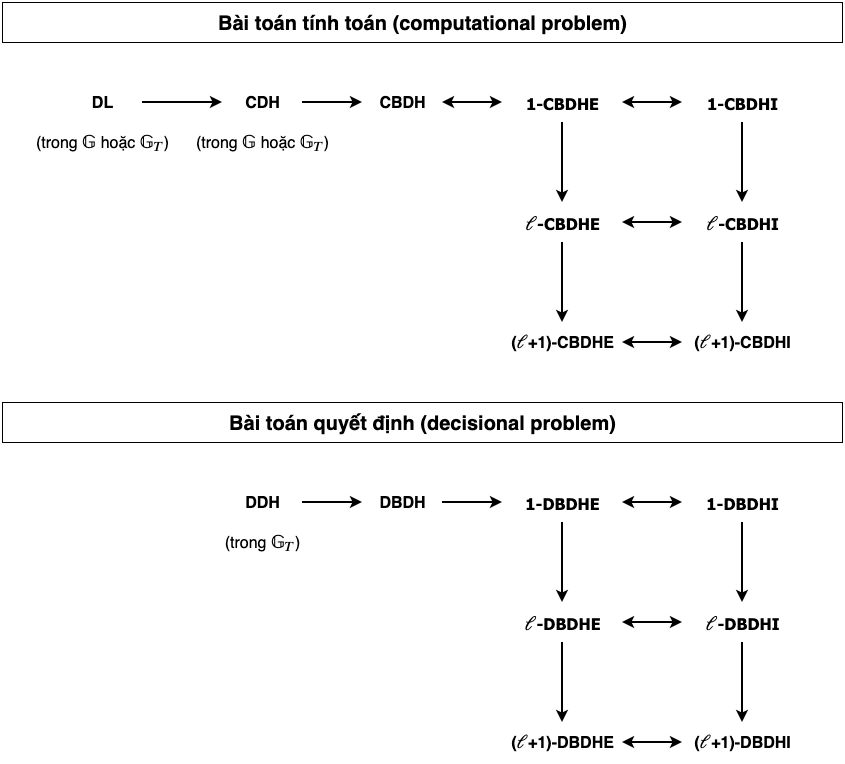
\includegraphics[width=\textwidth]{symmetric_problem_reduction.jpg}
				\centering
				\caption{Sơ đồ quy dẫn giữa các bài toán trên cặp ghép đối xứng}
				\label{fig:symmetric_reduction}
			\end{figure}
			%
			\begin{figure}[h]
				\captionsetup{font=normalsize}
				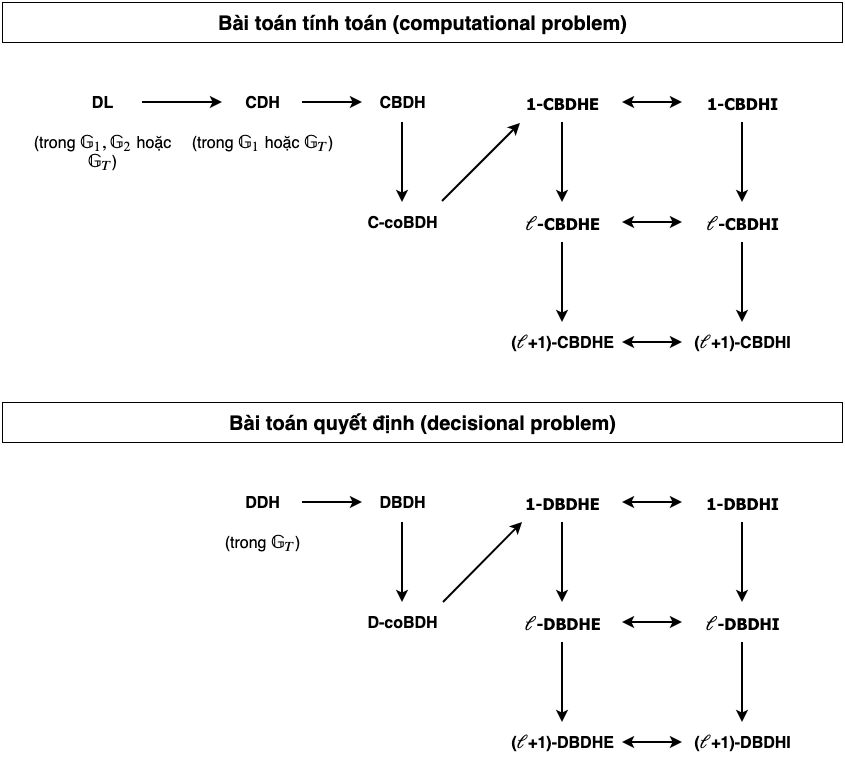
\includegraphics[width=\textwidth]{assymmetric_problem_reduction.jpg}
				\centering
				\caption{Sơ đồ quy dẫn giữa các bài toán trên cặp ghép bất đối xứng}
				\label{fig:assymmetric_reduction}
			\end{figure}
			%
			\begin{remark}
				Trong trường hợp $e$ là cặp ghép đối xứng với $\mathbb{G} = \mathbb{G}_1 = \mathbb{G}_2$ thì bài toán DDH \emph{ở trong $\mathbb{G}$} là dễ. Thật vậy, cho $g, g^x, g^y, u \in \mathbb{G}$, ta có thể kiểm tra các giá trị trên có tạo thành bộ Diffie-Hellman $(\text{tức}\ (g, g^x, g^y, g^{xy}))$ hay không bằng cách kiểm tra đẳng thức
				%
				\begin{equation}
					e(g, u) = e(g^x, g^y). \tag{*}\label{eq:check_ddh_tuple}
				\end{equation} \indent
				%
				Ta chứng minh \eqref{eq:check_ddh_tuple} thỏa khi và chỉ khi $u = g^{xy}$.
				\vspace{-\baselineskip}
				\begin{proof}[Chứng minh]
					Chiều đảo là hiển nhiên do tính song tuyến tính. Đặt $u = g^t$ với $t$ nào đó thuộc $\mathbb{Z}_p$. Nếu \eqref{eq:check_ddh_tuple} thỏa thì ta có
					\[
						e(g, g)^{xy} = e(g^x, g^y) = e(g, u) = e(g, g^t) = e(g, g)^t.
					\]
					Theo nhận xét \ref{remark:pairing.2} ở trên thì $e(g, g)$ là phần tử sinh của $\mathbb{G}_T$, suy ra $t \equiv xy \pmod{p}$. Dẫn đến $u = g^t = g^{xy}$ (để ý rằng $\mathbb{G}$ và $\mathbb{G}_T$ đều là nhóm cyclic cấp $p$).
				\end{proof}
				%
				\vspace{-\baselineskip}
				Việc bài toán DDH trong $\mathbb{G}$ không còn khó nữa không những không làm mất nguồn bài toán khó hay làm các lược đồ xây dựng trên cặp ghép suy yếu, mà trái lại lại trở thành một công cụ tốt để thiết kế lược đồ mật mã. Ví dụ ta có thể kiểm tra bản mã có hợp lệ không bằng cách kiểm một bộ bốn (gồm phần tử trong bản mã và dữ liệu đã có) có là bộ Diffie-Hellman hay không. Và quan trọng hơn, bài toán CDH trong $\mathbb{G}$ và DDH trong $\mathbb{G}_T$ (được tin là) vẫn khó dù cho có cặp ghép đối xứng. Vì thế giả định độ khó của những bài toán trên vẫn còn đứng vững.
			\end{remark}
	%
	\section{Tiêu chí đánh giá một hệ IBE}
		\begin{figure}[h] 
			\captionsetup{font=normalsize}
			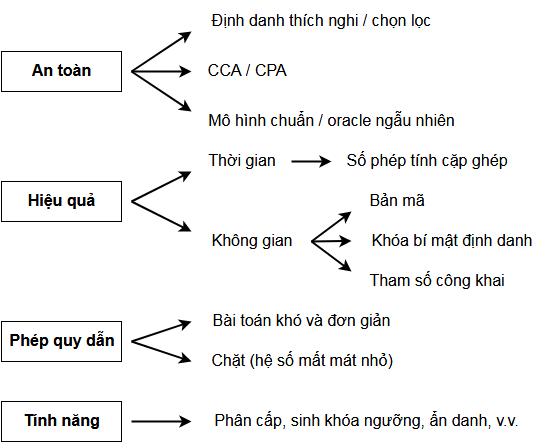
\includegraphics[width=0.8\textwidth]{ibe_criteria.png}
			\centering
			\caption{Tiêu chí đánh giá một hệ IBE}
		\end{figure}
		%
		\subsection{Tính an toàn}
			Trong các trò chơi an toàn nêu trên, người tấn công được chọn định danh mục tiêu sau một cách thích nghi (adaptive identity) tất nhiên có nhiều lợi thế hơn người phải chọn trước ngay từ đầu (selective identity). Và tương tự người được truy vấn giải mã (CCA) có lợi thế hơn người không được (CPA). Ta luôn muốn hệ mã phải an toàn trước người tấn công có nhiều sức mạnh và quyền hạn. Do đó mức an toàn chuẩn mực được hướng tới của một hệ (H)IBE là IND-ID-CCA.

			Một khía cạnh quan trọng không kém là việc hệ mã được chứng minh trong \textit{mô hình chuẩn} (standard model) hay \textit{mô hình oracle ngẫu nhiên} (random oracle model). Trong mô hình oracle ngẫu nhiên, các hàm băm mật mã được lý tưởng hóa thành hàm cho ra giá trị thực sự ngẫu nhiên. Vẫn còn nhiều nghi vấn về việc oracle ngẫu nhiên có thể hiện thực hóa được hay không, từ đó dẫn đến những nghi ngờ rằng một hệ mã an toàn trong mô hình oracle ngẫu nhiên có an toàn ngoài thực tế hay không. Nếu có thể thì một chứng minh an toàn trong mô hình chuẩn luôn được mong muốn hơn. Kết luận, một hệ (H)IBE đạt mức an toàn IND-ID-CCA với chứng minh trong mô hình chuẩn là mục đích tối thượng về tính an toàn của các nhà mật mã học.
		%
		\subsection{Độ hiệu quả}
			Với cặp ghép song tuyến tính trên đường cong elliptic (cũng là cặp ghép duy nhất sử dụng được trong mật mã cho đến giờ), chi phí phép tính cặp ghép là nặng hơn hẳn chi phí phép cộng điểm hay phép nhân điểm với số nguyên. Vì vậy, không ít nỗ lực được đầu tư vào việc tối ưu thuật toán tính cặp ghép và tìm đường cong elliptic thuận lợi để tính cặp ghép. Mặt khác, các nhà mật mã học luôn cố gắng hạn chế số lần tính cặp ghép trong lược đồ và tính sẵn nhiều nhất có thể. Xét riêng IBE, những hệ hiệu quả nhất mà sinh viên biết tới không cần tính cặp ghép nào khi sinh khóa, mã hóa và tính cặp ghép tối đa 4 lần khi giải mã, với điều kiện một số cặp ghép được tính sẵn khi thiết lập hệ thống. Lại có những hệ HIBE rất hiệu quả với số lần tính cặp ghép là hằng số (nhỏ), không phụ thuộc vào số cấp tối đa của hệ \cite{DBLP:conf/eurocrypt/BonehBG05}.

			Về không gian, trong một hệ (H)IBE có ba loại dữ liệu phải được vận chuyển và lưu trữ với nhiều bản sao trên toàn hệ thống là bộ tham số công khai, khóa bí mật định danh và bản mã. Khi thiết kế hệ mã, những nhà mật mã học ưu tiên việc giảm kích thước bản mã (hoặc khóa tùy vào ứng dụng). Kích thước các loại dữ liệu trên thường bị phóng đại theo số cấp tối đa trong hệ HIBE. Theo sinh viên biết thì đã có hệ HIBE đạt kích thước bản mã hằng số và hệ khác có kích thước khóa $\mathcal{O}(\sqrt{\ell})$ với $\ell$ là số cấp tối đa \cite{DBLP:conf/eurocrypt/BonehBG05}. Khi so sánh sơ lược độ hiệu quả không gian các hệ (H)IBE trên cặp ghép, các kích thước trên được đếm bằng số phần tử trong các cấu trúc đại số. Tuy nhiên khi triển khai thực tế, ta cần cân nhắc kích thước biểu diễn của một phần tử trong các nhóm để đưa ra lựa chọn các cấu trúc sử dụng và / hoặc áp dụng kỹ thuật làm giảm kích thước (chẳng hạn như băm).

			Với cặp ghép trên đường cong elliptic, trường hợp bất đối xứng cho ta cặp ghép với phần tử trong nhóm $\mathbb{G}_1$ nói ở trên có kích thước biểu diễn nhỏ hơn và nhiều lựa chọn họ đường cong phù hợp hơn trường hợp đối xứng. Vì vậy một hệ IBE vận hành và chứng minh an toàn được bằng bài toán trên cặp ghép tổng quát (không yêu cầu tính đối xứng) có thể áp dụng cặp ghép bất đối xứng để có những lợi ích trên hoặc cặp ghép đối xứng với mục đích nào đó khác.
		%
		\subsection{Phép quy dẫn}
			Giả sử ta đã chứng minh được phép quy dẫn từ bài toán C-BDH đến hệ IBE \scheme như sau: \\ \indent
			\textit{
			Giả sử giả định $(t, \varepsilon)$-C-BDH là đúng trong $(\mathbb{G}, \mathbb{G}_T, e)$. Khi đó hệ IBE \scheme là an toàn $(t', q_{id}, q_c, \varepsilon')$-IND-ID-CCA.}
			
			Gần như mọi trường hợp ta luôn có $t \geq t'$ và $\varepsilon \leq \varepsilon'$. Những sự chênh lệch này là mất mát phải đánh đổi trong phép quy dẫn, hiểu đơn giản là những chi phí tính toán phát sinh thêm trong quá trình chứng minh. Và ta mong muốn hai độ chênh lệch này phải càng nhỏ càng tốt. Một phép quy dẫn (hay chứng minh an toàn) được gọi là \textit{chặt} (tight reduction) nếu $t / t'$ và $\varepsilon' / \varepsilon$ đều thuộc $Poly(\lambda)$, với $\lambda$ là tham số an toàn của hệ mã. Nói cách khác, hai tỷ lệ này lớn nhất cũng chỉ được phép là hàm đa thức, nếu ta muốn chứng minh an toàn của hệ mã là đáng tin cậy. Thêm nữa, bài toán được quy dẫn phải khó (tương đối so với các bài khác), tự nhiên (có phát biểu "gọn gàng") và đã được nhiều người đánh giá, tìm cách giải.
		%
		\subsection{Những tính năng bổ sung}
			Sau khi đã đạt được tính an toàn, độ hiệu quả và phép quy dẫn như mong muốn trên một hệ IBE, điều tiếp theo các nhà mật mã học hướng tới là bổ sung thêm những tính năng như HIBE, cơ chế sinh khóa ngưỡng phi tương tác, tính ẩn danh người dùng, giới hạn số cấp sinh khóa, v.v. mà vẫn giữ được những ưu điểm sẵn có.
		
	%
	\section{Những công trình liên quan}\label{chap:2.related_works}
		Từ đây sinh viên xin gọi tắt tên các công trình bằng chữ cái đầu trong tên các tác giả. Đây cũng là cách gọi trong cộng đồng nghiên cứu. Sau hệ IBE đầu tiên trên cặp ghép của Boneh và Franklin \cite{DBLP:conf/crypto/BonehF01}, một loạt công trình liên quan đến IBE và cặp ghép ra đời các năm tiếp theo, cho thấy sự quan tâm rất lớn từ cộng đồng. Một hệ IBE đáng chú ý được xây dựng bởi Sakai và Kasahara \cite{DBLP:journals/iacr/SakaiK03} đạt độ hiệu quả rất tốt với duy nhất một lần tính cặp ghép trong toàn hệ (khi giải mã). Độ hiệu quả của hệ SK rất cạnh tranh dù là so sánh với những hệ mới hơn. Giữa hệ BF và hệ SK có một vài điểm giống nhau là thuật toán sinh khóa là đơn định (mỗi định danh chỉ có duy nhất một khóa hợp lệ), và an toàn IND-ID-CCA trong mô hình oracle ngẫu nhiên. Cũng trong \cite{DBLP:conf/crypto/BonehF01}, hai tác giả cũng mở ra vấn đề xây dựng một hệ IBE an toàn trong mô hình chuẩn. Sau đó, các nhà mật mã học nhận ra rằng ngẫu nhiên hóa thuật toán sinh khóa là điều kiện cần để có một hệ IBE an toàn trong mô hình chuẩn. Vì lý do đó các hệ IBE ra đời sau đều có thuật toán sinh khóa ngẫu nhiên và thực sự có chứng minh an toàn trong mô hình chuẩn. Tiêu biểu phải kể đến hai hệ IBE của Boneh và Boyen (gọi là BB\textsubscript{1}và BB\textsubscript{2}) \cite{DBLP:journals/joc/BonehB11}, hệ IBE của Waters \cite{DBLP:conf/eurocrypt/Waters05}, của Boneh, Boyen và Goh \cite{DBLP:conf/eurocrypt/BonehBG05}, và của Gentry \cite{DBLP:conf/eurocrypt/Gentry06}, với các mức an toàn đạt được khác nhau. Trong đó các hệ BB$_1$, Waters và BBG rất gần nhau về mặt đại số và có thể xây dựng các hệ HIBE lai (hybrid) dựa trên các hệ này, chi tiết xem tại \cite[mục 4.2]{DBLP:conf/eurocrypt/BonehBG05}.

		Về phía hệ phân cấp, cùng năm với đề xuất HIBE của Horwitz và Lynn \cite{DBLP:conf/eurocrypt/HorwitzL02}, Gentry và Silverberg \cite{DBLP:conf/asiacrypt/GentryS02} đã công bố một hệ HIBE là mở rộng của hệ BF. Hệ GS có tính năng rất tốt (và hiếm) là hạn chế được sự giám hộ khóa (đã nói ở mục \ref{subsec:key_escrow}), tuy nhiên tính hiệu quả là không cao và cũng như hệ BF, dùng tới oracle ngẫu nhiên để chứng minh an toàn. Hệ mã BB$_1$, Waters và BBG có thể mở rộng lên HIBE và hiệu quả hơn hệ GS.

		Trừ hệ mã của Gentry thì tất cả hệ (H)IBE nêu trên ban đầu đều chỉ đạt mức an toàn CPA. Và một số trong đó có thể áp dụng phép biến đổi để đạt CCA. Biến đổi Fujisaki-Okamoto \cite{DBLP:conf/crypto/FujisakiO99} có thể được áp dụng với hệ BF và SK để đạt mức an toàn IND-ID-CCA trong mô hình oracle ngẫu nhiên. Canetti, Halevi và Katz \cite{DBLP:conf/eurocrypt/CanettiHK04} đã đưa ra phương pháp xây dựng một hệ mã hóa khóa công khai an toàn IND-CCA không cần oracle ngẫu nhiên từ một hệ IBE an toàn IND-sID-CPA trong mô hình chuẩn bất kỳ kết hợp thêm một hệ \textit{chữ ký một lần} (one-time signature). Sau đó Boneh và Katz \cite{DBLP:conf/ctrsa/BonehK05} cải tiến độ hiệu quả bằng cách thay chữ ký một lần bằng MAC. Mặt khác, Boyen, Mei và Waters \cite{DBLP:conf/ccs/BoyenMW05} đưa ra tiếp cận không cần sử dụng thêm bất kỳ mật mã nguyên thủy nào ngoài chính hệ IBE, đổi lại mất đi tính tổng quát là chỉ áp dụng được với hệ BB$_1$, Waters và BBG. Nếu áp dụng với một trong ba hệ mã này, ba biến đổi trên đều cho ta một hệ $\ell$-HIBE an toàn IND-sID-CCA trong mô hình chuẩn từ một hệ $(\ell + 1)$-HIBE với $\ell$ là số cấp tối đa. Bên cạnh đó, Boneh, Boyen và Halevi \cite{DBLP:conf/ctrsa/BonehBH06} cũng đã mở rộng biến đổi Canetti-Halevi-Katz cho tính năng ngưỡng, có thể biến một hệ IBE ngưỡng (threshold IBE) an toàn CPA thành hệ mã hóa khóa công khai ngưỡng an toàn CCA.

		Dựa vào những kết quả nghiên cứu, việc đạt được an toàn CCA có vẻ dễ hơn là đạt được an toàn trong trò chơi định danh chọn sau, và đặc biệt khó khi nói đến HIBE kể cả khi dùng đến oracle ngẫu nhiên. Sở dĩ là do các phép quy dẫn thường bị mất mát một thừa số lũy thừa theo chiều sâu phân cấp $\ell$, và nếu $\ell$ là hàm đa thức theo tham số an toàn $\lambda$ thì phép quy dẫn không còn ý nghĩa. Do đó $\ell$ phải bị giới hạn nhỏ hơn hàm logarit theo $\lambda$ trong các hệ HIBE này. Sinh viên cũng nhấn mạnh rằng đã có một số kết quả xây dựng được hệ HIBE an toàn hoàn toàn \cite{DBLP:conf/tcc/GentryH09, DBLP:conf/crypto/Waters09, DBLP:conf/tcc/LewkoW10, DBLP:journals/jise/HuWXY14}, tuy nhiên các hệ này đều hoặc là quá phức tạp, hoặc thiếu hiệu quả, hoặc dựa trên giả định chưa được nhiều người kiểm chứng. Do đó sinh viên chọn không trình bày các hệ trên trong khóa luận này.
		
		Sẽ là không quá khi nói rằng, đích đến cuối cùng của nghiên cứu mã hóa dựa trên định danh là tạo ra một con ``dao Thụy Sỹ'' trong mật mã, là một hệ HIBE an toàn IND-ID-CCA trong mô hình chuẩn, hiệu quả về thời gian, kích thước bản mã, khóa bí mật và tham số công khai hằng số, dựa trên bài toán khó và tự nhiên, cộng thêm các tính năng phụ như không bị giám hộ khóa, ẩn danh, hỗ trợ sinh khóa có ngưỡng ở mọi cấp.

		Kết thúc chương, sinh viên xin trình bày so sánh giữa một số hệ (H)IBE. Độ hiệu quả sẽ được đánh giá chi tiết ở chương \ref{chap:5}. Với độ hiệu quả tốt hơn các hệ HIBE khác do kích thước bản mã hằng số, cộng thêm với việc áp dụng được biến đổi BMW để lên an toàn CCA, hỗ trợ sinh khóa có ngưỡng ở cấp 0, hệ mã BBG rõ ràng có ưu điểm hơn các hệ khác. Vì những lý do trên, sinh viên quyết định chọn hệ mã BBG để trình bày trong khóa luận này.
		%
		\newpage
		\subimport{./}{ibe_general_comparison_table.tex}
	%
	% Reset default lengths
	\import{../}{default_lengths.tex}
\end{document}
